% !TeX document-id = {3aec7d78-4a32-4a0f-a5ca-01214b5f7293}
% +---------------------------------------------------------------+
% | Author :    Noémie Plancherel, HEIG-VD
% | Date :      04.03.22
% +---------------------------------------------------------------+

\documentclass[a4paper,11pt,twoside,openright]{book} % Type du document

% compiler avec : pdflatex, bibtex, pdflatex, pdflatex
% !TeX TXS-program:compile = txs:///pdflatex/[--shell-escape]

% +---------------------------------------------------------------+
% | Language
% +---------------------------------------------------------------+
\usepackage[T1]{fontenc}
%\usepackage[mono=false]{libertine}
\usepackage[utf8]{inputenc}
\usepackage[french]{babel}
\usepackage{tablefootnote}
\usepackage{hyperref}
\usepackage{caption}
\usepackage{xcolor}
\newif\ifisconfidential	\isconfidentialfalse

\newif\ifisdraft\isdraftfalse



% +---------------------------------------------------------------+
% | Paramètres
% +---------------------------------------------------------------+

\newcommand{\TBtitle}{Gestionnaires de mots de passe : quelle sécurité ? }
\newcommand{\TBsubtitle}{}%laisser vide si pas de sous-titre
\newcommand{\TByear}{2022}
\newcommand{\TBacademicYears}{2022-2023}

\newcommand{\TBdpt}{Département des Technologie de l'information et de la communication (TIC)}
\newcommand{\TBfiliere}{Filière Télécommunications}
\newcommand{\TBorient}{Orientation Sécurité de l'information}

\newcommand{\TBauthor}{Noémie Plancherel}
\newcommand{\TBsupervisor}{Prof. Sylvain Pasini}

% Confidentiel?
% uncomment if confidential / comment if not confiential
% \isconfidentialtrue

\newcommand{\TBresumePubliable}{
Dans ce travail... Ceci est le résumé publiable...
}

% +---------------------------------------------------------------+



% +-[set path]-------------------------------------+
\usepackage{template/TB-style}
\usepackage{template/TB-macros}
\usepackage{template/TB-template}
%\graphicspath{images/}


\begin{document}

\frontmatter
\pagestyle{empty}

% TITLE and template
% +---------------------------------------------------------------+

\TBmaketitle

\pagestyle{frontmatter}

\TBsecondTitle

\TBpreambule

\TBauthentification


% Cahier des charges
% +---------------------------------------------------------------+
% +---------------------------------------------------------------+
% | Author :    Noémie Plancherel, HEIG-VD
% | Date :      April 1st, 2022
% +---------------------------------------------------------------+


\chapter{Cahier des charges}



\section*{Résumé du problème}
De nos jours, les gestionnaires de mots de passe sont des outils très fréquemment utilisés. En effet, une bonne pratique est d'utiliser un mot de passe par service. De cette manière, si un service est compromis et le mot de passe divulgué, cela n'implique pas les autres. Il est également très important de choisir un mot de passe fort qui ne contient pas d'éléments facilement prévisibles et qui pourrait être brute-forcé rapidement. 

Les gestionnaires de mots de passe permettent principalement de faciliter le stockage des mots de passe qui demandent d'être de plus en plus longs et complexes, de manière à ne pas les réutiliser. Ils permettent également d'ajouter une couche sécuritaire aux mots de passe en les stockant de manière sécurisée et en offrant la possibilité de générer des mots de passe forts.

Ces applications offrent plusieurs fonctionnalités sous la forme de différents types;  elles permettent, entre autres, l'utilisation du cloud afin de stocker les mots de passe sur les serveurs du fournisseur pour faciliter la synchronisation des données entre plusieurs devices (mobile, montre, navigateur, etc.). Certains gestionnaires de mots de passe sont également fréquemment utilisés au sein d'entreprises pour permettre le partage de données. Les entreprises vont généralement utiliser une solution self-hosted où ils auront leur propre infrastructure et stockage. Il existe des extensions de navigateur  qui proposent le remplissage automatique de mots de passe dans les formulaires de connexion. Enfin, il y a également des applications en local qui vont limiter leur utilisation à un seul appareil.

Étant donné que les utilisateurs se reposent grandement sur les gestionnaires de mots de passe, il est important de s'assurer que ces logiciels satisfassent un certain nombre de principes de sécurité ainsi qu'une implémentation robuste afin d'éviter tout vol ou perte de données. 

\section*{Objectifs}
Ce travail de bachelor vise à comprendre les menaces d'un gestionnaire de mots de passe, premièrement de manière générique, puis sur des produits spécifiques, sélectionnés à la suite d'une étude complète, en analysant la sécurité sous différents angles (stockage, mémoire, réseau, cryptographie, etc.). 

Il est réalisé en deux parties distinctes; une première partie qui est une étude approfondie et complète sur les gestionnaires de mots de passe. Elle permet d'analyser les menaces des différents type de gestionnaires de mots de passe et de présenter les exigences sécuritaires qu'il serait nécessaire de garantir. Elle va également se concentrer sur une étude de marché avec une comparaison de plusieurs gestionnaires de mots de passe existants sous différents aspects.

La deuxième partie du travail se concentrera tout d'abord sur la sélection de quelques candidats (environ 4) en fonction de critères établis au préalable. Ensuite, le but est d'évaluer la sécurité de manière complète de chaque gestionnaire de mot de passe sélectionné; chaque élément choisi est analysé et évalué en fonction de différents critères comme les choix cryptographiques utilisés, le stockage, ou encore l'architecture de l'application.

%\begin{enumerate}
%	\item cloud
%	\item local - application desktop
%	\item extension de navigateur
%	\item closed-source
%\end{enumerate}

\subsection*{Livrables}
Les délivrables seront les suivants :
\begin{enumerate}
\item Une documentation contenant :
	\begin{itemize}
	\item Présentation des différents types de gestionnaires de mots de passe
	\item Étude de marché
	\item Une analyse de menaces de différents types de gestionnaires de mots de passe
	\item Spécification des exigences sécuritaires à garantir
	\end{itemize}
\item Analyse sécuritaire des quelques candidats représentatifs (environ 4) :
	\begin{itemize}
	\item Sélection de candidats pour la suite du travail
	\end{itemize}
chaque analyse se décomposera ainsi :
	\begin{itemize}
		\item Sélection de critères d'analyse
		\item Analyse complète de chaque aspect
		\item Rapport des faiblesses trouvées au fabricant
	\end{itemize}
\item Synthèse des résultats
\item Comparaison entre chaque candidat
\end{enumerate}

\subsection*{Déroulement}
En se référant aux dates officielles émises par la HEIG-VD, le travail de bachelor débute le 21 février 2022 et se termine au plus tard le 16 septembre 2022. Il y a 3 dates clés incluant des rendus:
\begin{itemize}
	\item \textbf{16 mai 2022} - rendu du rapport intermédiaire
	\item \textbf{29 juillet 2022} - rendu du rapport final
	\item \textbf{22 août au 16 septembre 2022} - soutenance du travail de bachelor
\end{itemize}

Etant donné, que la soutenance du travail implique l'intervention d'un expert, la date doit être définie entre tous les intervenants.

Le volume du travail de bachelor est de 15 crédit ECTS, soit 450 heures. Le rapport intermédiaire représente 150 heures de travail. Au niveau de la répartition de la charge de travail, cela représente ~13h/semaine jusqu'au 19 juin, puis 45h/semaine jusqu'au rendu, soit le 29 juillet. 



% Planning
% +---------------------------------------------------------------+
% +---------------------------------------------------------------+
% | Author :    Noémie Plancherel, HEIG-VD
% | Date :      April 1st, 2022
% +---------------------------------------------------------------+


\chapter{Planning}
Le travail de bachelor sera séparé en plusieurs tâches et sous-tâches différentes qui permettront de répartir plus facilement le travail sur des périodes de plusieurs semaines. Ci-dessous, le planning détaillé avec toutes les tâches : 

\begin{enumerate}
	\item Préparation
	\begin{itemize}
		\item Rédaction du cahier des charges
		\item Planification
		\item Recherches initiales et introduction
	\end{itemize}
	\item Étude de marché
		\begin{itemize}
			\item Recherche et explication des différents types de gestionnaires de mots de passe
			\item Comparaison des fonctionnalités, du prix et des plateformes disponibles
			\item Analyse du marché actuel et de la demande
			\item Récapitulatif 
		\end{itemize}
	\item Étude sécuritaire
		\begin{itemize}
			\item Présentation de la sécurité implémentée dans les gestionnaires de mots de passe
			\item Identification et analyse des menaces potentielles
			\item Rédaction des exigences sécuritaires
		\end{itemize}
	\item Sélection
		\begin{itemize}
			\item Mise en place des critères de sélection des candidats
			\item Sélection des candidats
		\end{itemize}
	\item Analyse sécuritaire (pour chaque candidat)
		\begin{itemize}
			\item Identification et rédaction des critères d'analyse 
			\item Analyse sécuritaire de chaque aspect
		\end{itemize}
	\item Synthèse (pour chaque candidat)
		\begin{itemize}
			\item Synthèse des résultats
			\item Rapport des faiblesses au fabricant
		\end{itemize}
	\item Synthèse générale
		\begin{itemize}
			\item Comparaison de tous les résultats
			\item Conclusion du travail
		\end{itemize}
	\item Documentation
		\begin{itemize}
			\item Rédaction du rapport
			\item Lecture / visualisation de documents
			\item Tenue d'un journal de travail
		\end{itemize}
\end{enumerate}

Un diagramme de Gantt a également été effectué afin de pouvoir visualiser le planning et ajouter des périodes de temps :
\begin{figure}[h!]
	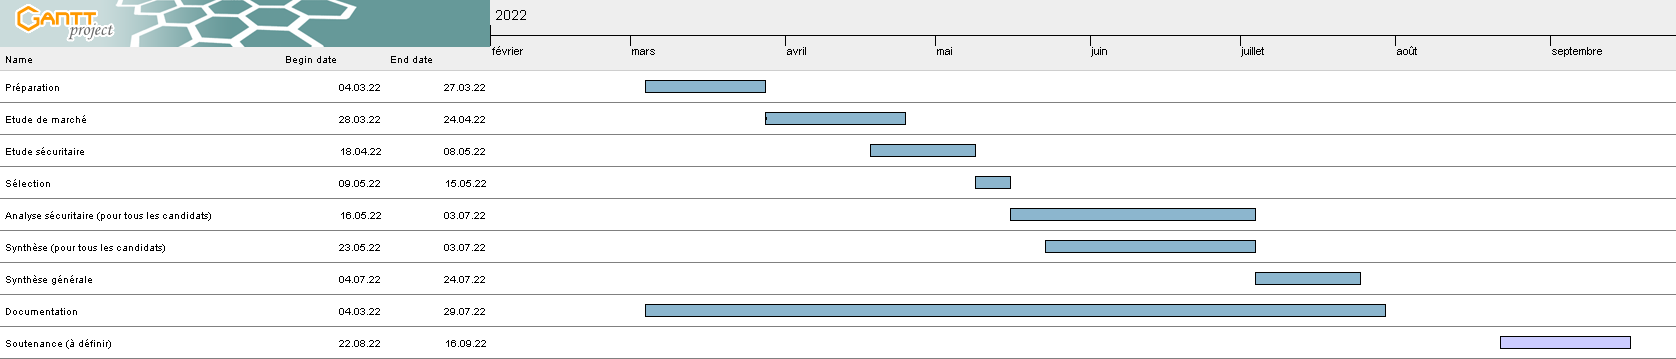
\includegraphics[width=15.5cm]{images/planning.png}
	\caption{Planning du travail de Bachelor}
\end{figure}


% TOC
% +---------------------------------------------------------------+
\tableofcontents
\clearpage


% Content
% +---------------------------------------------------------------+

\mainmatter
\pagestyle{plain}

% +---------------------------------------------------------------+
% | Author :    Noémie Plancherel, HEIG-VD
% | Date :      18.04.2022
% +---------------------------------------------------------------+


\chapter{Introduction}
\label{ch:intro}

Pour un utilisateur lambda, il peut être difficile de se souvenir de tous ses mots de passe tout en s'assurant d'en utiliser un différent pour chaque service afin d'éviter tout vol de données. Typiquement dans ces situations, nous allons naturellement utiliser des mots de passe simples, qui sont facilement mémorisables. Comme, par exemple, utiliser son prénom et sa date de naissance, "123456" ou encore "qwerty". De plus, il est plus simple d'utiliser le même mot de passe pour chacun de ses comptes, afin d'en mémoriser uniquement un seul. 

Cependant, même si l'unique mot de passe qu'on utilise est fort et aléatoire, il n'est pas garanti à 100\% qu'on soit la cible d'aucun attaquant et si une attaque est réalisée, toutes nos données personnelles sont exposées.

Ainsi, dans ce genre de cas, les gestionnaires de mots de passe interviennent et peuvent faciliter le quotidien de la plupart des utilisateurs. 

\section{Fonctionnement général}

Les gestionnaires de mots de passe sont des applications multi-plateformes qui vont permettre de stocker des informations sensibles telles que des mots de passe, numéros de carte de crédit ou encore des fichiers confidentiels. On peut les comparer à des coffres forts.  

Ces derniers proposent un \textit{master password} ou une \textit{master key} qui va permettre d'accéder à l'ensemble des données secrètes. En conséquence, la sécurité repose sur un seul mot de passe principal, ce qui est très bénéfique pour les utilisateurs car ils n'ont qu'un mot de passe à retenir. Une fois l'accès à l'application, l'utilisateur a la possibilité de stocker des données, générer des mots de passe ainsi que se connecter à des services en ligne (remplissage de formulaire d'identification automatique).

Les gestionnaires de mots de passe sont disponibles en plusieurs types différents en fonction du besoin de l'utilisateur et des fonctionnalités proposées. 

\section{Types}

\subsection{Cloud}
Les gestionnaires de mots de passe dans le cloud sont proposés pour un usage personnel ainsi qu'un usage professionnel. Les mots de passe entrés dans le coffre fort vont directement être stockés sur les serveurs du constructeur et ils seront également chiffrés sur ces derniers. Aucun stockage n'est effectué en local.

Le cloud va permettre aux utilisateurs d'avoir accès à leurs données sur n'importe quel device (ordinateur, mobile, montre) et à tout moment. De plus, toutes les données vont être synchronisées sur tous les devices connectés.

À propos de la sécurité, elle repose entièrement sur le provider de l'application car toutes les informations sont stockées sur leurs propres serveurs.

\subsection{Local}
Les applications en local s'installent sur le desktop ou sur le mobile de l'utilisateur. Ces gestionnaires de mots de passe fonctionnent indépendamment et sont offline. Ces produits peuvent donc être utilisés sur une seule machine, par conséquence la synchronisation n'est pas proposée pour ce type de password manager. 

Toutes les données sensibles sont directement stockées et chiffrées sur le device. La sécurité est plutôt bonne comparé à la solution cloud car c'est du hors-ligne, cependant si on récupère / vole le device, la sécurité devient plus faible car il y aurait la possibilité d'avoir accès aux informations sensibles du gestionnaire de mots de passe, via notamment une gestion de mémoire mal gérée. 

Il y a également une solution \textit{on-premise} (ou \textit{self-host}) qui permet d'utiliser sa propre infrastructure locale pour héberger toutes les données du gestionnaire de mots de passe. Les fonctionnalités offertes sont les mêmes que pour les solutions cloud mais le prix est en général plus cher et l'application plus orientée professionnelle.

\subsection{Navigateur}
Le dernier type de gestionnaire de mots de passe sont ceux qui sont basés sur le navigateur (\textit{browser-based}). Les navigateurs les plus populaires, tels que Firefox, Safari ou Chrome offrent ce gestionnaire de mots de passe qui est directement inclu dans ces derniers.
Ils vont faciliter la gestion et la sauvegarde de mots de passe de comptes de sites web. Il y a également la possibilité de synchroniser toutes les données stockées entre tous les devices qui supportent le navigateur en question (Chrome, Firefox, Safari, etc.).

Pour certains navigateurs, les informations sont stockées et chiffrées en local sur le device de l'utilisateur. Si la synchronisation est activée, les données seront également stockées dans le cloud sur les serveurs du constructeur. Un problème de sécurité importante, et la disponibilité des mots de passe sur le navigateur, si aucun master password n'est configuré et qu'on a accès à la machine, les mots de passe sont accessibles en clair sur le navigateur.


% +---------------------------------------------------------------+
% | Author :    Noémie Plancherel, HEIG-VD
% | Date :      18.04.2022
% +---------------------------------------------------------------+



\chapter{Étude de marché}
\label{ch:etude_marche}
Ce chapitre vise à étudier les différentes fonctionnalités offertes par les gestionnaires de mots de passe en les comparant entre plusieurs produits sélectionnés et en établissant un tableau afin d'avoir une meilleure vue d'ensemble.

Nous allons également analyser les différents prix des applications ainsi que présenter où en est le marché actuel afin d'étudier la popularité de ces dernières.

Pour l'étude de marché, les gestionnaires de mots de passe sélectionnés seront: \textit{LastPass}\footnote{\href{https://www.lastpass.com/}{https://www.lastpass.com/}}, \textit{Dashlane}\footnote{\href{https://www.dashlane.com/}{https://www.dashlane.com/}}, \textit{1Password}\footnote{\href{https://1password.com/}{https://1password.com/}}, \textit{KeePass}\footnote{\href{https://keepass.info/}{https://keepass.info/}}, \textit{Bitwarden}\footnote{\href{https://bitwarden.com/}{https://bitwarden.com/}}, \textit{NordPass}\footnote{\href{https://nordpass.com/}{https://nordpass.com/}}, \textit{RoboForm}\footnote{\href{https://www.roboform.com/}{https://www.roboform.com/}}, \textit{Keeper}\footnote{\href{https://www.keepersecurity.com/}{https://www.keepersecurity.com/}}.

Ils ont été sélectionnés en se basant sur leur popularité sur le marché ainsi qu'à la suite de lecture d'articles concernant les meilleurs gestionnaires de mots de passe \cite{BPM22}\cite{gallagher19}\cite{MSPM22}\cite{PM22}.
\section{Fonctionnalités}
Ci-après, une liste des fonctionnalités disponibles dans les gestionnaires de mots de passe. Cette énumération se base sur toutes les fonctionnalités citées sur les websites des différents des \textit{password manager}. \\
\begin{enumerate}
\item Stockage d'informations personnelles (cartes de crédit, passeport, contrats, etc.)
\item Remplissage automatique des formulaires en ligne (auto-complétion)
\item Partage de données entre plusieurs utilisateurs (par exemple, partage d'informations d'identifications entre une famille)
\item Générateur de mots de passe forts
\item Surveillance de la fuite de données ou données compromises
\item Alerte en cas de données compromises
\item Synchronisation de données entre devices (cloud)
\item Authentification à double facteurs
\item Self-hosting
\item Support prioritaire
\item Connexion à l'aide de facteurs biométriques (\textit{fingerprint} ou \textit{facial recognition}) ou d'un pin
\item Possibilité de stockage des secrets en local

\end{enumerate}
Ci-dessous un tableau récapitulatif qui indique quels gestionnaires de mots de passe offre quelles fonctionnalités. 
\begin{longtable}[h]{|c|c|c|c|c|c|c|c|c|c|c|c|c|}
	\hline
	Application & 1 & 2 & 3 & 4 & 5 & 6 & 7 & 8 & 9 & 10 & 11 & 12 \\
	\hline
	LastPass & $\times$ & $\times$ & $\times$! & $\times$* & $\times$* &  $\times$*& $\times$ & $\times$ & & $\times$* & $\times$* & $\times$ \\
		\hline
	Dashlane & $\times$* & $\times$ & $\times$! & $\times$ & $\times$* & $\times$ & $\times$* & $\times$! & & & & $\times$ \\
		\hline
	1Password\footnote{L'application est totalement payante et différents abonnements sont proposés \label{1p}} & $\times$* & $\times$* & $\times$* & $\times$* & & $\times$* & $\times$* & $\times$* & & $\times$* & & $\times$* \\
			\hline
	KeePass \footnote{En général, nécessite l'installation de plugins supplémentaires afin de profiter de toutes les fonctionnalités} & $\times$ & $\times$ &  & $\times$ & $\times$ & & & $\times$ & $\times$ & & $\times$ & $\times$\\
		\hline
	Bitwarden &  & $\times$  & $\times$! & $\times$ & $\times$* & $\times$* & $\times$ & $\times$! & $\times$* &  $\times$* & $\times$!& $\times$ \\
	\hline
	NordPass & $\times$ & $\times$ & $\times$*  & $\times$ & $\times$* & & $\times$ & $\times$ & $\times$* & $\times$* & $\times$ & $\times$\\
	\hline
	RoboForm & $\times$ & $\times$ & $\times$* & $\times$ & & $\times$ & $\times$* & $\times$* & $\times$* & $\times$* & & $\times$\\
	\hline
	Keeper\footnote{Se référer à la note de bas de page \ref{1p}} & $\times$* & $\times$*\footnote{Extension \textit{KeeperFill}} & $\times$* & $\times$* &$\times$* & $\times$* & $\times$* &$\times$* &$\times$* & $\times$* & $\times$* &  $\times$* \\
	\hline
	\caption{Fonctionnalités proposées par les candidats}
\end{longtable} 
$\times$ : L'application propose cette fonctionnalités \\
\textbf{*}\hspace{0.1cm} : Fonctionnalité proposée mais avec un version premium (payante) \\
\textbf{!}\hspace{0.18cm} : Limitations avec une version gratuite \\

Sur tous les candidats sélectionnés, nous remarquons que la plupart offre la majorité des fonctionnalités énumérées plus haut. Nous constatons que l'offre des constructeurs de gestionnaires de mots de passe est assez variée et répond à la demande des particuliers et des entreprises.
\section{Plateformes}
Cette partie va permettre de visualiser sur quelles plateformes les gestionnaires de mots de passe sélectionnés sont supportés. \\
\begin{longtable}[h]{|c|c|c|c|c|c|c|}
	\hline
	Application & Windows & MacOS & Linux & Android & iOS & Navigateur  \\
	\hline
	LastPass & $\times$ & $\times$ & $\times$ & $\times$ & $\times$ &  $\times$\\
		\hline
	Dashlane & $\times$ & $\times$ & $\times$! & $\times$ & $\times$ & $\times$  \\
		\hline
	1Password & $\times$ & $\times$ & $\times$ & $\times$ & $\times$& \\
	\hline
	KeePass & $\times$ & $\times$* & $\times$*  & $\times$* & $\times$* &  $\times$*  \\
		\hline
	Bitwarden & $\times$ & $\times$  & $\times$ & $\times$ & $\times$ & $\times$  \\
		\hline
	NordPass & $\times$ & $\times$ & $\times$  & $\times$ & $\times$ &  \\
		\hline
	RoboForm & $\times$ & $\times$ & $\times$! & $\times$ & & $\times$ \\
		\hline
	Keeper & $\times$ & $\times$ & $\times$ & $\times$ &$\times$ & $\times$ \\
		\hline
	\caption{Plateformes supportées par les différentes applications}
\end{longtable}
$\times$ : L'application est supportée sur ces plateformes \\
\textbf{*}\hspace{0.1cm} :  Des applications (ou des paquets) compatibles avec KeePass Password Safe non-officielles mais contribuées existent \\
\textbf{!}\hspace{0.18cm} : Utilisation via des extensions de navigateur \\

Même si un gestionnaire supporte toutes les plateformes indiquées, il est nécessaire d'aller vérifier les conditions d'utilisation du système, c'est-à-dire les versions des plateformes afin de s'assurer que l'application fonctionnera quand même. 

Cependant, nous constatons que la majorité des applications sont disponibles sur les plateformes les plus courantes, et même si elles ne le sont pas, il y a souvent une solution non-officielle (notamment pour KeePass) ou via le navigateur qui existe.
\section{Prix}
Nous allons passer brièvement en revue les prix proposés par les gestionnaires de mots de passe. Chaque application propose leurs propres gammes de prix avec également des abonnements possibles pour les particuliers, familles ou entreprises. 
\subsection{Particuliers}
Pour la plupart des applications, nous pouvons retrouver 3 gammes de prix; Gratuit, Premium, Famille. L'offre familiale va être plus cher car les gestionnaires de mots de passe sont conçus pour pouvoir avoir plusieurs gestionnaires chiffrés individuels différents. 
Les tarifs ci-dessous sont exprimés en mensualités. \\
\begin{longtable}[h]{|c|c|c|c|}
		\hline
	Application & Gratuit & Premium & Famille \\
		\hline
	LastPass & \$0 & \$3 & \$4  \\
		\hline
	Dashlane & \$0 & \$3.99 & \$5.99 n \\
		\hline
	1Password & non & \$2.99 & \$4.99  \\
		\hline
	KeePass\footnote{gratuit et open-source} & \$0 & non & non   \\
		\hline
	Bitwarden & \$0 & <\$1 & \$3.33   \\
		\hline
	NordPass & \$0 & \$1.84 & \$4.99  \\
	\hline
	RoboForm & \$0 & \$1.99 & \$3.99    \\
	\hline
	Keeper & non & \$2.92 & \$6.25  \\
		\hline
			\caption{2.3 Tarifs pour particuliers}
\end{longtable}
\subsection{Entreprises}
Les entreprises ont quant à elle des prix différents dû à leurs besoins spécifiques où ils pourraient avoir besoin d'un devis personnel afin de choisir l'abonnement qui convient au mieux à leur infrastructure.
\begin{longtable}[h]{|c|c|c|c|}
	\hline
	Application & Gratuit & Premium & Famille \\
	\hline
	LastPass & \$0 & \$3 & \$4  \\
	\hline
	Dashlane & \$0 & \$3.99 & \$5.99 n \\
	\hline
	1Password & non & \$2.99 & \$4.99  \\
	\hline
	KeePass\footnote{gratuit et open-source} & \$0 & non & non   \\
	\hline
	Bitwarden & \$0 & <\$1 & \$3.33   \\
	\hline
	NordPass & \$0 & \$1.84 & \$4.99  \\
	\hline
	RoboForm & \$0 & \$1.99 & \$3.99    \\
	\hline
	Keeper & non & \$2.92 & \$6.25  \\
	\hline
	\caption{2.3 Tarifs pour particuliers}
\end{longtable}
\section{Marché actuel}
prix sur le marché, popularité, lier l'augmentation des cyberattaques avec le covid-19 + peur de perdre ses données
\section{Récapitualtif de l'étude}


% +---------------------------------------------------------------+
% | Author :    Noémie Plancherel, HEIG-VD
% | Date :      18.04.2022
% +---------------------------------------------------------------+

\chapter{Étude sécuritaire}
\label{ch:etude_secu}

Ce chapitre est dédié à toute l'analyse sécuritaire des gestionnaires de mots de passes en général. Nous allons dans un premier temps décrire comment ces applications sont sécurisées en fonction de leur type, puis justifier l'importance d'une forte sécurité suite à l'augmentation de la demande des entreprises et des particuliers.

Dans un second temps, nous allons identifier et analyser toutes les menaces existantes et / ou potentielles des \textit{password manager} en mettant en avant les failles actuellement connues des constructeurs et les conséquences de ces dernières ou des faiblesses qui pourraient survenir à tout moment (par exemple des cyberattaques).

Finalement, nous allons rédiger toutes les exigences sécuritaires que doivent respecter les gestionnaires de mots de passe afin que ces dernières garantissent une utilisation sûre qui évite des pertes ou vol de données.

\section{Implémentation de la sécurité dans les gestionnaires de mots de passe}

Dans cette section, afin de se baser sur des gestionnaires de mots de passe déjà existants et de pouvoir comparer les différentes sécurités implémentées, nous allons reprendre les 8 candidats sélectionnés dans la partie \hyperref[ch:etude_marche]{\textit{étude de marché}}, c'est-à-dire; \textit{LastPass}, \textit{Dashlane}, \textit{1Password}, \textit{KeePass}, \textit{Bitwarden}, \textit{NordPass}, \textit{RoboForm} et \textit{Keeper}. Toutes les informations citées sont basées sur les \textit{security whitepapers} des constructeurs\cite{lastpasssecurity}\cite{dashlanesecurity}\cite{1passwordsecurity}\cite{keepasssecurity}\cite{bitwardensecurity}.

Les gestionnaires de mots de passe sélectionnés fonctionnent tous de la même manière, au final cette méthode est plutôt classique dans les architectures des applications. Un \textit{master password} (qui est seulement connu par l'utilisateur) est généré ou entré par l'utilisateur et va permettre le déverrouillage de l'application et le chiffrement / déchiffrement de toutes les données stockées. 



- utilisation de la mémoire et stockage des secrets
\subsection{Les gestionnaires cloud-based}
\subsection{Les gestionnaires browser-based}
\subsection{Les gestionnaires en local}
\subsection{Partage d'informations}
est-ce que c'est pertinent de parler de ça à ce moment ?
\subsection{Perte du master password}
\subsection{3 états du gestionnaire de mot de passe}

\subsubsection{Etat \textit{Not Running}}
\subsubsection{Etat \textit{Unlocked State}}
en expliquant chaque état et pour l'état unlock expliquer comment est géré le master password, avec des schemas
explication pour extension de navigateur, local et cloud-based
\subsubsection{Etat \textit{Locked State}}

+ facteurs biométriques !

\subsection{Algorithmes cryptographiques}
- les algos utilisés pour le chiffrement et auth des données 
\subsection{L'importance d'une forte sécurité}
\colorbox{pink}{\parbox{15cm}{à voir si utile}}
\section{Analyse des menaces}
\subsection{Failles connues des constructeurs}
\colorbox{pink}{\parbox{15cm}{à voir si je devrais pas les ajouter dans le chapitre de l'analyse de chaque gestionnaire sélectionné}}
\subsection{Conséquences d'une quelconque faiblesse}
\colorbox{pink}{\parbox{15cm}{à voir si utile, mais les conséquences seront sûrement soulignées lorsque je ferai l'analyse de menaces de toute manière}}
\section{Exigences sécuritaires à respecter}

% +---------------------------------------------------------------+
% | Author :    Noémie Plancherel, HEIG-VD
% | Date :      04.10.2022
% +---------------------------------------------------------------+

\chapter{Analyse de menaces}
\label{ch:analyse_menaces}

Ce chapitre a pour but d'identifier et analyser toutes les menaces existantes et / ou potentielles des \textit{password managers} en les modélisant en suivant un certain processus afin d'avoir une meilleure vision des risques.

Puis, nous allons rédiger toutes les exigences sécuritaires que doivent respecter les gestionnaires de mots de passe afin que ces dernières garantissent une utilisation sûre qui évite des pertes, un vol de données, une usurpation d'identité, des accès aux services, etc.

\section{Modélisation de menaces}
Afin de modéliser correctement les menaces, nous allons suivre la norme ISO 27005\cite{ISO27005}. Cela va nous permettre de séparer la modélisation en un processus avec plusieurs étapes comme suit:

\begin{enumerate}
	\item Établissement du contexte, qui inclut
	\begin{itemize}
		\item Objectifs des gestionnaires de mots de passe
		\item Hypothèses et exigences de sécurité
		\item Actifs à haute valeur 
		\item Data Flow Diagram
		\item Définition des critères d'analyse
	\end{itemize}
	\item Identification des risques
		\begin{itemize}
		\item Identification des biens
		\item Identification des menaces
		\item Identification des contrôles
		\item Identification des vulnérabilités
		\item Identification des conséquences
	\end{itemize}
	\item Analyse des risques
	\item Évaluation des risques
	\item Traitement des risques
	\item Documentation 
\end{enumerate}
La dernière étape ne sera pas explicitement abordée car elle vise à documenter le modèle de menaces que nous allons établir.

Pour chaque étape du processus, nous allons aborder les 3 types de gestionnaires que nous avons cité précédemment: local-based, browser-based et cloud/local-based. Étant donné que les applications browser-based et cloud/local-based fonctionnent les deux en local et en cloud avec la synchronisation de données, nous pouvons nous baser sur deux catégories uniquement; les gestionnaires \textbf{local-based} et \textbf{cloud/local-based}. 

Nous allons également nous baser sur le processus de modélisation de menaces de OWASP\cite{owasp}.

Il est intéressant de mélanger les deux méthodologies car la norme ISO est plus axée sur une gestion des risques alors que OWASP se base sur une modélisation des menaces. Les deux ont des points communs notamment au niveau de la description et la décomposition de l'application, néanmoins la norme ISO va plus en profondeur en identifiant tous les risques possibles (vulnérabilités, menaces, conséquences, etc.). OWASP a également ses avantages en schématisant le flux de données à l'aide de DFDs (\textit{Data Flow Diagram}) et en catégorisant les menaces avec le modèle STRIDE. \newpage

\subsection{Définition des critères}

Avant de commencer, nous allons définir les différents critères et niveaux pour évaluer l'impact des événements (les conséquences), la probabilité d'événement, la sévérité des vulnérabilités ainsi que l'évaluation des risques. Ces niveaux seront réutilisés pour l'identification des risques dans la suite de l'analyse de menaces.

\begin{table}[H]
	\begin{tabular}{llc}
		\hline
		Échelle  & Description                                                                                                                                                                                               & Valeur   \\ \hline
		Aucune   & La vulnérabilité ne présente aucune sévérité                                                                                                                                                              & 0        \\
		Bas      & \begin{tabular}[c]{@{}l@{}}La vulnérabilité a peu d'impact sur l'entreprise et demande un\\ accès physique ou local au système\end{tabular}                                                               & 0.1-39   \\
		Moyen    & \begin{tabular}[c]{@{}l@{}}En général, elle demande à l'attaquant d'être sur le même réseau \\ que la victime et elle demande les privilèges utilisateurs pour \\ effectuer une exploitation\end{tabular} & 4.0-6.9  \\
		Haut     & \begin{tabular}[c]{@{}l@{}}La vulnérabilité est difficile à exploter, peut être une élévation de \\ privilèges et peut amener à une importante perte de données ou \\ de temps d'arrêt\end{tabular}       & 7.0-8.9  \\
		Critique & \begin{tabular}[c]{@{}l@{}}Exploitation de vulnérabilités au niveau root, l'attaquant n'a pas\\ besoin d'être authentifié ou avoir des connaissances sur la victime\end{tabular}                          & 9.0-10.0 \\ \hline
	\end{tabular}
	\caption{Scores de sévérité basés sur CVSS v3.1}
\end{table}

\begin{table}[H]
	\centering
	\resizebox{\textwidth}{!}{\begin{tabular}{llc}
			\hline
			Échelle        & Description                                                                                                                                                                                                    & Valeur \\ \hline
			Négligeable    & L'impact sur l'entreprise est négligeable                                                                                                                                                                      & 0      \\
			Mineur         & \begin{tabular}[c]{@{}l@{}}L'effet sur les biens de l'entreprise est limité, comme entraîner des \\ pertes financières mineures ou entraîner des dommages mineures \\ aux actifs de l'entreprises\end{tabular} & 1      \\
			Modéré         & \begin{tabular}[c]{@{}l@{}}L'effet sur les biens peut être grave, les effets causés sur les biens \\ seront considérés comme importants\end{tabular}                                                           & 2      \\
			Important      & L'effet sur les biens de l'entreprise peut être grave à catastrophique                                                                                                                                         & 3      \\
			Catastrophique & \begin{tabular}[c]{@{}l@{}}On s'attend à ce que la menace ait de multiples effets graves à \\ catastrophiques sur les biens de l'entreprise\end{tabular}                                                       & 4      \\ \hline
	\end{tabular}}
	\caption{Impact des menaces sur l'entreprise}
\end{table}

\begin{table}[H]
	\centering
	\begin{tabular}{llc}
		\hline
		Échelle      & Description                                            & Valeur \\ \hline
		Rare         & La probabilité que l'événement arrive est rare         & 0      \\
		Peu probable & La probabilité que l'événement arrive est peu probable & 1      \\
		Possible     & La probabilité que l'événement arrive est possible     & 2      \\
		Probable     & La probabilité que l'événement arrive est probable     & 3      \\
		Certain      & La probabilité que l'événement arrive est certain      & 4      \\ \hline
	\end{tabular}
	\caption{Probabilités d'événements}
\end{table}

Pour l'évaluation des risques, il est important de prendre en considération la probabilité d'événements et les conséquences sur l'entreprise afin de définir une échelle d'évaluation de risques. Nous utilisons une matrice de risques basée sur une étude quantitative\cite{matrix}.

\begin{figure}[H]
	\centering
	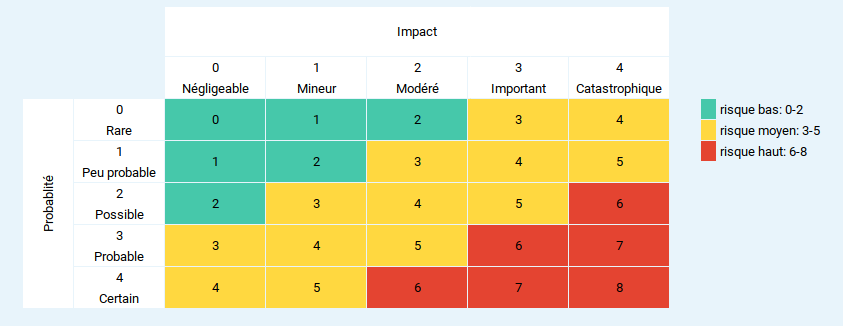
\includegraphics[width=15.5cm]{images/risque_evaluation.png}
	\centering
	\caption{Critères d'évaluation des risques \label{Critères d'évaluation des risques}}
\end{figure}

\subsection{Établissement du contexte}
Dans cette section, nous allons comprendre les applications et comment interagissent les gestionnaires de mots de passe avec les entités externes. Au final, nous allons établir un \textit{Data Flow Diagram} (DFD) qui va nous permettre de présenter tous les chemins différents du système en mettant en avant les vulnérabilités potentielles.

\textbf{Objectifs du système}

Comme cité plusieurs fois, l'objectif principal d'un gestionnaire de mots de passe est de stocker de manière \textbf{sûre} des informations sensibles, le plus souvent des identifiants, mais également la possibilité de stocker des notes, des informations bancaires, contrats, etc. Ils offrent également la fonctionnalité de générer des mots de passe forts et d'auto-compléter les champs de connexion. 

Tout dépend, du gestionnaire de mots de passe, ils peuvent offrir une fonctionnalité de backup, afin de sauvegarder le coffre-fort et de garantir une perte minimale de données au cas où. Il existe également la fonctionnalité de partage de données entre utilisateurs.

Pour les applications qui fonctionnent avec le cloud et qui ne sont pas 100\% offline, l'utilisateur a la possibilité de synchroniser ses données entre appareils (desktop, mobile, navigateur, smartwatch). 

\textbf{Hypothèses de sécurité}

On peut émettre plusieurs hypothèses de sécurité afin de mettre en avant ce que doit assurer le gestionnaire de mots de passe pour être considéré comme sûr. Nous allons lister les hypothèses afin que cela soit le plus clair possible :

\begin{itemize}
	\item Données du gestionnaire soient chiffrées et protégées en RAM, sur le disque ainsi que lors de communications avec les serveurs. Nous définissons les données comme étant le coffre-fort, avec tous les identifiants, les clés et le master password. 
	\item Serveurs de confiance
\end{itemize}

Ceux-ci étant les plus importants afin de garantir la meilleure sécurité possible sur l'application, nous irons plus en détails dans la section sur les exigences sécuritaires.

\textbf{Actifs de valeurs}

Nous pouvons à présent définir les actifs (\textit{assets}) des gestionnaires de mots de passe, qui représentent les éléments qui ont de la valeur et qui demandent une importante protection. 

Tout d'abord, un actif à haute valeur est le \textbf{gestionnaire de mot passe} qui représente l'application. Cette dernière peut être sous forme d'application desktop, extension de navigateur ou application mobile. Un utilisateur ou un administrateur devrait pouvoir se connecter à l'application pour avoir accès à son coffre-fort.

Ensuite, un autre bien important est \textbf{le coffre-fort} qui contient tous les identifiants, notes, informations bancaires, etc. stockées par l'utilisateur, qui peut être représenté comme une base de données. Le bien principal sont donc les données, qui sont chiffrées et protégées. Un utilisateur devrait ainsi avoir l'habilité d'avoir accès à son coffre-fort en clair et de pouvoir y ajouter au minimum des identifiants.

Un actif qu'on peut également ajouter est le \textbf{master password} entré l'utilisateur pour déverrouiller le gestionnaire de mots de passe et avoir accès à son coffre-fort. Cet élément est très important car il va permettre de dériver les clés de chiffrement et ainsi, de pouvoir avoir accès au coffre-fort en clair.

Un autre actif à haute valeur sont les \textbf{clés}. Nous incluons dans cet actif les clés de chiffrement ainsi que les clés privées lors du partage de données entre utilisateurs. Nous pouvons ajouter le processus de génération de clés.

Dans le cadre de gestionnaires de mots de passe cloud/local-based qui ne fonctionnent pas en mode offline, nous voulons protéger les données des \textbf{serveurs du constructeur}. Le processus de transfert de données, c'est-à-dire la communication, est également important car les données doivent impérativement être protégées. Nous pouvons inclure les fonctionnalités de synchronisation de données et le partage de données entre utilisateur, qui demandent de passer par les serveurs du constructeur.

Un asset important à ajouter sont les \textbf{données partagées} entre utilisateurs lors de la fonctionnalité de partage. La ou les données échangées doivent être sécurisées afin de ne pas les exposer à n'importe quel utilisateur. 

Finalement, nous pouvons ajouter comme dernier actif, les fichier de \textbf{backups} qui devraient être chiffrés et protégés sur les devices de l'utilisateur ou des serveurs du provider.

À présent, pour effectuer une analyse de menaces la plus claire et structurée possible, nous allons séparer l'application en plusieurs parties comme suit:

\begin{enumerate}
	\item[\textbf{M1}] Coffre-fort standalone, local-based (haut-niveau)
	\item[\textbf{M2}] Fonctionnalité de backup
	\item[\textbf{M3}] Fonctionnalité de synchronisation (pour les gestionnaires cloud-based)
	\item[\textbf{M4}] Fonctionnalité de partage
	\item[\textbf{M5}] Sécurité de l'application et ses composants (bas-niveau)
\end{enumerate}

Pour chaque étape, nous identifierons et analyserons les risques pour couvrir tous les aspects et les fonctionnalités d'un gestionnaire de mots de passe. UN code d'identification a été ajouté afin de mieux organiser l'analyse.

Nous ferons un récapitulatif à la fin en évaluant tous les risques définis sur toutes les étapes et en listant toutes les contre-mesures nécessaires à prendre.
\newpage

\subsection{M1 Application haut-niveau}

La première partie qu'on analyse, définit une application standalone toute simple, qui est un gestionnaire de mots de passe qui ne fonctionne qu'en local et qui interagit avec aucune entité externe. Premièrement, nous avons effectué un DFD (\textit{Data Flow Diagram}) afin de constater les processus principaux de l'application :

\begin{figure}[H]
	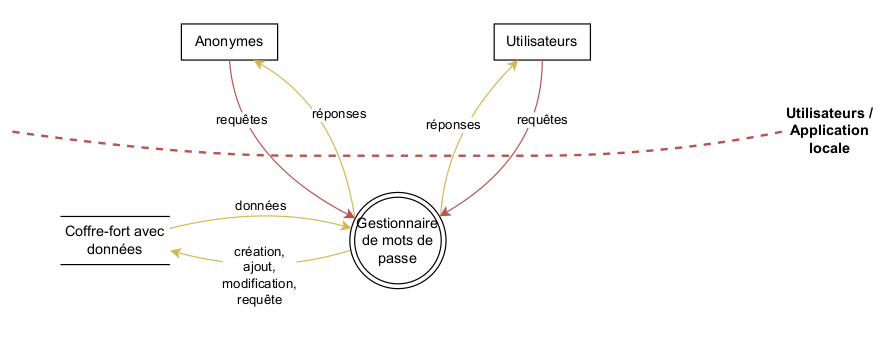
\includegraphics[width=13cm]{images/dfd_local.png}
	\centering
	\caption{Data Flow Diagram pour les gestionnaires M1}
\end{figure}

\subsubsection{Identification des risques}
Cette section va nous servir à déterminer ce qui peut se produire pour causer un dommage et à comprendre comment, où et pourquoi l'incident peut se produire. 

Afin d'établir une étude complète, nous allons premièrement identifier les biens, menaces (avec les sources de menaces et les scénarios), les contrôles, les vulnérabilités ainsi que les conséquences sur l'entreprise.

\textbf{Identification des biens}

Nous avons déjà identifié les actifs plus-haut dans l'analyse, cependant nous allons identifier les actifs présents dans une application standalone. De plus, nous allons ajouter un code pour les identifier et les référencer plus tard dans l'identification des risques.

\begin{table}[H]
	\centering
	\resizebox{\textwidth}{!}{\begin{tabular}{lll}
		\hline
		Code & Bien                                & Description                                                           \\ \hline
		A1   & Gestionnaire de mots de passe & L'application du gestionnaire de mots de passe                      \\
		A2   & Coffre-fort                     & Base de données avec toutes les informations stockées                \\
	    A3  & Master password                   & Mot de passe principal afin de déchiffrer le coffre-fort               \\
		\hline
	\end{tabular}}
\caption{Biens des gestionnaires de mots de passe M1}
\end{table}
\textbf{Identification des sources de menaces}

Nous allons identifier toutes les sources de menaces possibles des gestionnaires de mots de passe avec leurs motivations (uniquement si c'est de source humaine) afin de pouvoir mettre en avant les différents scénarios de menaces.

\begin{table}[H]
	\centering
	\begin{tabular}{cll}
		\hline
		Code & Source de menace                & Motivations                               \\ \hline
		S1   & Hackers & Amusement, gloire, challenge, argent, ego \\
		S2   & Script kiddies                  & Curiosité, ego, argent, amusement         \\
		S3   & Concurrent                      & Espionnage, réutilisation de contenu      \\
		S4   & Cybercrime                      & Argent, destruction de données            \\
		S5   & Accident humain                 & -                                         \\
		S6   & Problèmes techniques            & -                                         \\ \hline
	\end{tabular}
\caption{Sources de menaces des gestionnaires de mots de passe M1}
\end{table}

Ci-dessous, se trouve un tableau avec différents scénarios d'attaques par rapport aux biens que nous avons défini précédemment. Nous nous basons sur le modèle STRIDE\footnote{\href{https://owasp.org/www-community/Threat_Modeling_Process}{https://owasp.org/www-community/Threat\_Modeling\_Process}} afin de définir les types de menaces. 
\begin{table}[H]
		\centering
	\resizebox{\textwidth}{!}{\begin{tabular}{ccclll}
			\hline
			& Code & Code du bien & Scénario de menace                                                                                                            & Type de menace                & Source de menace    \\ \hline
			2 & T2   & A1, A3           & \begin{tabular}[c]{@{}l@{}}Key-logger installé sur le device de l'utilisateur \\ et qui sniff le master password\end{tabular} & \textit{Elevation of privileges}    & S1, S2, S4        \\
			2 & T2   & A1           & \begin{tabular}[c]{@{}l@{}}Utilisateur non-déconnecté de son compte \\et attaquant a accès au device\end{tabular}                                                                                     & \textit{Elevation of privileges}      & S1, S2, S4, S5   \\
			3 & T1   & A1           & Mauvais mécanisme d'authentification                                                                                          & \textit{Spoofing}    & S1, S2, S4, S6    \\
			4 &T3   & A1           & Lecture du presse-papier                                                                                                      & \textit{Information disclosure}    & S1, S2, S4       \\                                                                                
			5 & T1   & A1           & \begin{tabular}[c]{@{}l@{}}Coffre-fort compromis dû à des identifiants volés\\ sur d'autres sites\end{tabular}                & \textit{Spoofing}      & S1, S2, S4, S5   \\
			6 & T3   & A2           & \begin{tabular}[c]{@{}l@{}}Récupération du coffre-fort et déchiffrement\\ dû à un algorithme trop simple\end{tabular}  & \textit{Information disclosure}    & S1, S2, S4      \\
			7 & T6   & A2           & Injection SQL dans la base de données utilisateur                                                                                                                           & \textit{Tampering}           & S1, S2, S4 	 \\  
			8 & T1   & A3           & Brute-force sur le master password                                                                                            & \textit{Spoofing}      & S1, S2, S4, S5  \\			
			9 & T1   & A3           & Phishing par mail pour récupérer le master password  	  & \textit{Spoofing}   & S1, S2, S3, S4    \\		                                                                                                         
			\\\\	\hline 
			\multicolumn{6}{l}{A1 = Gestionnaire de mots de passe | A2 = Coffre-fort | A3 = Master password}\\ \hline
	\end{tabular}}
\caption{Scénarios et types d'attaques possibles sur applications M1}
\end{table}

\textbf{Identification des contrôles}

Une étape importante lors de l'identification des risques est d'identifier les contrôles qui existent déjà sur les applications sur lesquelles nous basons notre analyse de risques. Étant donné, que notre étude est plutôt générale car elle ne se base pas sur un seul gestionnaire de mots de passe, nous allons énumérer les contrôles qui ont été entrepris afin de baisser le niveau de risque. Nous parlerons en détails des contrôles effectués lors de la seconde partie du travail.

Étant donné que dans cette partie, nous nous concentrons sur une application basique qui ne fonctionne qu'en local et que nous abordons pas le bas-niveau, nous n'irons pas en détails au niveau des contrôles. 

Ce qui existe déjà pour éviter des attaques sur mots de passe sont des critères qui sont, pour la plupart des gestionnaires, imposés par le constructeur. Ces critères exigent par exemple d'avoir un certain nombre de caractères afin d'avoir un master password fort.

Au niveau de la protection du keylogger, aucune protection n'est réellement implémentée, à part utiliser l'application dans environnement sécurisé comme \textit{Secure Desktop} sur Windows. Pour la protection du presse-papier, certaines applications (comme Keepass) mettent à disposition une fonctionnalité pour enlever les données sensibles du presse-papier et de la mémoire après un certain moment.

Pour le coffre-fort, la plupart des gestionnaires de mots de passe proposent un chiffrement fort du coffre-fort afin de protéger au mieux les données, afin que même si ce dernier est volé, la personne malveillante ne puisse pas le déchiffrer et récupérer les données stockées.

\textbf{Identification des vulnérabilités}

Pour chaque actif identifié au préalable, nous allons analyser les vulnérabilités qui pourraient être présentes. Nous allons également ajouter la sévérité de la vulnérabilité. 

\begin{table}[H]
	\centering
		\resizebox{\textwidth}{!}{\begin{tabular}{cll}
				\hline
				Bien                   & Vulnérabilité                                                                                                          & Sévérité de la vulnérabilité   \\ \hline
				A1                     & Temps de session long                                                                                                  & Critique                     \\
				A1                     & Presse-papier non nettoyé après un certain temps                                                                       & Moyen                         \\
				A1                     & 2FA pas proposé par défaut                                                                                             & Haut                        \\
				A1                     & Aucune authentification effectuée                                                                                      & Moyen                        \\
				A1                     & Génération de mots de passe faibles                                                                                    & Haut                       \\
				A1                     & Manque de contrôle des entrées utilisateurs                                                                                                   & Haut                           \\		
				A2                     & Possibilité d'avoir des entrées dans le coffre-fort qui ont le même mot de passe                                                                                                  & Haut                           \\	
				A3                     & Master password trop faible                                                                                            & Haut                        \\	
				A3                     & Master password non unique                                                                                             & Bas                         \\												
				\\ \\ \hline
					\multicolumn{3}{l}{A1 = Gestionnaire de mots de passe}\\ \hline
			\end{tabular}}
	\caption{Vulnérabilités présentes dans les gestionnaires de mots de passe M1}
\end{table}

\textbf{Identifications des conséquences}

Il est également important d'identifier les conséquences qui pourraient être causés par un incident. Nous allons définir par bien actif quelles sont les conséquences qu'ils pourraient y avoir sur l'entreprise lors d'une perte de confidentialité, intégrité ou disponibilité. Pour cela, nous allons nous référer au tableau qui définit différents scénarios de menaces. Nous allons également ajouter les éléments que nous souhaitons garantir pour chaque bien.

\begin{table}[H]
	\centering
\resizebox{\textwidth}{!}{	\begin{tabular}{lll}
		\hline
		Bien                     & Conséquences     & Garanties                                                                                             \\ \hline
		Application (A1)         & Perte de réputation et d'image      & Disponibilité, intégrité                                                                           \\
		Base de données (A2)     & Perte de réputation et d'image, perte de données        & Confidentialité, intégrité des données             \\
		Master password (A3)     & Perte de réputation et d'image, perte de données        & Confidentialité, intégrité des données             \\
		 \hline
	\end{tabular}}
\caption{Conséquences des menaces sur l'entreprise}
\end{table}

\subsubsection{Analyse des risques}
L'objectif de cette section est d'estimer la probabilité des incidents et les conséquences pour les biens qu'ils menacent. Pour ce faire, nous allons faire une analyse de risque qualitative ce qui va nous permettre de faire une première analyse de risques assez générale afin de nous permettre d'aller plus en détails dans la seconde partie du travail de Bachelor.

Ainsi, nous allons analyser l'impact des conséquences ainsi que la probabilité que chaque scénario d'attaque identifié puisse se produire. Pour cela, nous allons utiliser plusieurs notations différentes; pour les conséquences nous aurons les niveaux suivants:

	\begin{table}[H]
		\centering
		\resizebox{\textwidth}{!}{\begin{tabular}{cclllll}
				\hline 
		Bien & Menace & Scénario                                                                                                                     & Impact des conséquences & Probabilité  & Niveau de risque \\ \hline
		A1, A3   & T2     & \begin{tabular}[c]{@{}l@{}}Key-logger installé sur le device de l'utilisateur\\ et qui sniff le master password\end{tabular} & Important               & Possible     & Moyen            \\
		A1   & T2     & \begin{tabular}[c]{@{}l@{}}Utilisateur non-déconnecté de son compte\\ et attaquant a accès au device\end{tabular}            & Important               & Probable     & Haut             \\
		A1   & T1     & Mauvais mécanisme d'authentification                                                                                         & Modéré                  & Rare         & Bas            \\
		A1   & T3     & Lecture du presse-papier                                                                                                     & Modéré                  & Probable     & Moyen            \\

		A1   & T1     & \begin{tabular}[c]{@{}l@{}}Coffre-fort compromis dû à des identifiants \\ volés sur d'autres sites\end{tabular}              & Mineur                  & Possible     & Moyen              \\
		A2   & T3     & \begin{tabular}[c]{@{}l@{}}Récupération de la base de données et déchiffrement\\ dû à un algorithme trop simple\end{tabular} & Important          & Peu probable & Moyen            \\
		A2   & T6     & Injection SQL dans la base de données                                                                                 & Important          & Peu probable     & Moyen             \\
		A3   & T1     & Brute-force sur le master password                                                                                           & Important               & Certain      & Haut            \\	
		A3   & T1     & Phishing par mail pour récupérer le master password                                                                                    & Modéré                  & Possible     & Moyen            \\			
	 \\\\ \hline 
			\multicolumn{6}{l}{A1 = Gestionnaire de mots de passe | A2 = Base de données | A3 = Master password}\\ 
				\multicolumn{6}{l}{T1 = Spoofing | T2 = Elevation of privileges | T3 = Information Disclosure | T4 = Denial of service | T5 = Equipment failure | T6 = Tampering}\\ 
			\hline
	\end{tabular}}
\caption{Analyse des risques de chaque scénario de menaces pour M1}
\end{table}
\newpage
\subsection{M2 Backup}

Cette partie concerne la fonctionnalité de backup des coffre-forts qui est offerte par tous les gestionnaires de mots de passe. Il y a plusieurs techniques de sauvegardes qui existent; une solution proposée par les applications en local est l'exportation des données avec un fichier CSV (toutes les données sont en claires) ou un fichier chiffré. Sinon, il y a la possibilité d'effectuer des sauvegardes sur les seveurs du provider, seulement s'il s'agit d'un gestionnaire cloud-based. Un DFD a été défini ci-dessous afin de mieux comprendre le processus de sauvegarde:

\begin{figure}[H]
	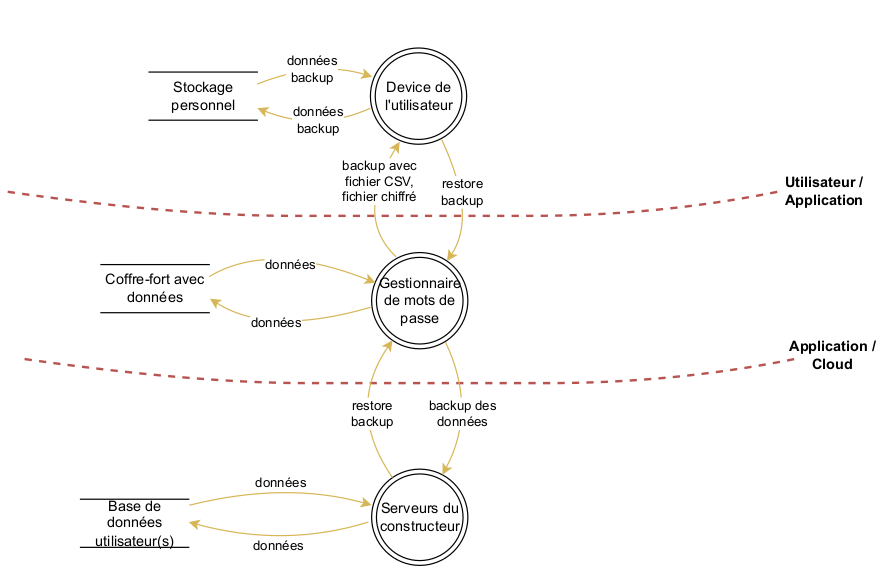
\includegraphics[width=14.5cm]{images/dfd_backup.png}
	\centering
	\caption{Data Flow Diagram pour les applications M2}
\end{figure}

\subsubsection{Identification des risques}

Nous allons procéder exactement comme la section précédente, nous allons premièrement identifier les biens, menaces (avec les sources de menaces et les scénarios), les contrôles, les vulnérabilités ainsi que les conséquences sur l'entreprise afin d'établir une étude complète.

\textbf{Identification des biens}

Ci-dessous les biens présents lors du processus de sauvegarde de données dans un gestionnaire de mots de passe local-based ou cloud/local-based.

\begin{table}[H]
	\centering
	\resizebox{\textwidth}{!}{\begin{tabular}{lll}
			\hline
			Code & Bien                                & Description                                                           \\ \hline
			A1   & Serveurs du constructeur                     & Serveurs qui stockent les données des utilisateur dans le cloud               \\
			A2 & Sauvegardes & Fichiers ou emplacements contenant les sauvegardes des données \\
			\hline
	\end{tabular}}
	\caption{Biens des gestionnaires de mots de passe M2}
\end{table}
\textbf{Identification des sources de menaces}

Nous allons identifier toutes les sources de menaces possibles qui pourraient survenir dans le cadre de backups de données d'un gestionnaire de mots de passe. 

\begin{table}[H]
	\centering
	\begin{tabular}{cll}
		\hline
		Code & Source de menace                & Motivations                               \\ \hline
		S1   & Hackers & Amusement, gloire, challenge, argent, ego \\
		S2   & Script kiddies                  & Curiosité, ego, argent, amusement         \\
		S3   & Concurrent                      & Espionnage, réutilisation de contenu      \\
		S4   & Cybercrime                      & Argent, destruction de données            \\
		S5   & Accident humain                 & -                                         \\
		S6   & Problèmes techniques            & -                                         \\ \hline
	\end{tabular}
	\caption{Sources de menaces des gestionnaires de mots de passe M2}
\end{table}

Ci-dessous, se trouve un tableau avec différents scénarios d'attaques. Nous utilisons le modèle STRIDE afin de définir tous les types de menaces. 

\begin{table}[H]
	\centering
	\resizebox{\textwidth}{!}{\begin{tabular}{ccclll}
			\hline
			& Code & Code du bien & Scénario de menace                                                                                                            & Type de menace                & Source de menace  \\ \hline
			1 & T3   & A1           & \begin{tabular}[c]{@{}l@{}}Communication non chiffrée entre gestionnaire\\ de mots de passe et serveurs\end{tabular}                                                                                  & \textit{Information Disclosure}          & S1, S2, S4, S6   \\
			2 & T3   & A1           & MITM (Interception de données non-chiffrées)                                                                                  & \textit{Information Disclosure}          & S1, S2, S4, S6   \\
			3 & T4   & A1           & DoS                                                                                                                           & \textit{Denial of service}           & S1, S2, S4, S6    		\\
			4 & T5   & A1           & Perte des données utilisateurs dû à un serveur down                                                                                                                           & \textit{Equipment failure}           & S5, S6   	\\
			5 & T3   & A2          & Récupération du backup en clair sur le device du client                                                                                  & \textit{Information Disclosure}          & S1, S2, S3, S4, S6   \\	
			6 & T3   & A2          & Sauvegarde corrompue                                                                                 & \textit{Information Disclosure}          & S5, S6   \\	
			7 & T3   & A2          & Perte de la sauvegarde sur device utilisateur                                                                                 & \textit{Information Disclosure}          & S1, S2, S3, S4, S6   \\	
						8 & T3   & A2           & Vols de backups non protégés sur le serveur                                                                                  & \textit{Information disclosure} & S1, S2, S4, S6         \\
						
			\\\\	\hline 
			\multicolumn{6}{l}{A1 = Serveurs du constructeur | A2 = Sauvegardes}\\ \hline
	\end{tabular}}
	\caption{Scénarios et types d'attaques possibles sur M2}
\end{table}

\textbf{Identification des contrôles}

Dans cette partie, nous nous concentrons uniquement sur la fonctionnalité de backup, ainsi, la liste des contrôles existants n'est pas grande. 

L'unique contrôle que l'on peut citer, qui est fait de manière indirect, est que la sauvegarde sur les serveurs du constructeur est entièrement chiffrée. Étant donné que dans leurs bases de données utilisateurs, le coffre-fort est toujours chiffré grâce au \textit{Zero-knowledge}, naturellement le backup le sera aussi. Cela nous garantit que les données ne sont pas connues des serveurs et sont protégées de quelconques attaques sur ces derniers.

Au niveau du device utilisateur, il est possible d'effectuer des contrôles mais c'est à l'utilisateur de s'assurer que les données sont stockées dans un emplacement sécurisé et à l'abri de toute manipulation malveillante.

\textbf{Identification des vulnérabilités}

Pour chaque actif identifié au préalable, nous allons analyser les vulnérabilités qui pourraient être présentes. Nous allons également ajouter la sévérité de la vulnérabilité. 

\begin{table}[H]
	\centering
	\resizebox{\textwidth}{!}{\begin{tabular}{cll}
			\hline
			Bien                   & Vulnérabilité                                                                                                          & Sévérité de la vulnérabilité   \\ \hline
			A1                     & Backup non effectué sur les serveurs                                                                                            & Critique                        \\
			A1                     & Communication non chiffrée                                                                                                  & Critique                     \\
			A1                     & Infrastructure des serveurs pas assez stable                                                                      & Haut                         \\
			A1                     & \begin{tabular}[c]{@{}l@{}}Infrastructure des serveurs du constructeur pas \\   protégée à quelconques intrusions physiques \end{tabular}                                                                      & Bas                         \\
			A2                    & Manque de chiffrement dans les sauvegardes sur serveurs ou device utilisateur                                                                                            & Critique                        \\
			A2                    & Sauvegarde stockée dans un répertoire personnel non protégé                                                                                    & Moyen                        \\
			A2                     &  Sauvegarde CSV stockée dans un emplacement non sécurisé                                                                                 & Moyen                       \\			
			\\ \\ \hline
			\multicolumn{3}{l}{A1 = Serveurs du constructeur | A2 = Sauvegardes}\\ \hline
	\end{tabular}}
	\caption{Vulnérabilités présentes dans les gestionnaires de mots de passe M2}
\end{table}

\textbf{Identifications des conséquences}

Pour chaque bien défini plus haut, nous allons ajouter les conséquences qu'il pourrait y avoir dans le cas d'attaques, ainsi que ce que nous souhaitons garantir.

\begin{table}[H]
	\centering
	\resizebox{\textwidth}{!}{	\begin{tabular}{lll}
			\hline
			Bien                     & Conséquences     & Garanties                                                                                             \\ \hline
			Serveurs du constructeur (A1)         & Perte de réputation et d'image, pertes de données      & Disponibilité, intégrité, confidentialité                                                                           \\
			Sauvegardes (A2)     & Perte de réputation et d'image, perte de données        & Confidentialité, intégrité des données             \\ \hline
	\end{tabular}}
	\caption{Conséquences des menaces sur l'entreprise}
\end{table}

\subsubsection{Analyse des risques}
Ainsi, dans cette partie, nous allons analyser l'impact des conséquences ainsi que la probabilité que chaque scénario d'attaque identifié puisse se produire. Pour cela, nous allons utiliser plusieurs notations différentes; pour les conséquences nous aurons les niveaux suivants:

\begin{table}[H]
	\centering
	\resizebox{\textwidth}{!}{\begin{tabular}{cclllll}
			\hline 
			Bien & Menace & Scénario                                                                                                                     & Impact des conséquences & Probabilité  & Niveau de risque \\ \hline
			A1   & T3           & \begin{tabular}[c]{@{}l@{}}Communication non chiffrée entre gestionnaire\\ de mots de passe et serveurs\end{tabular}                                                                          &    Catastrophique            & Peu probable      &      Moyen       \\
			A1   & T3           & MITM (Interception de données non-chiffrées) &      Catastrophique          &   Peu probable  &     Moyen        \\
			A1   & T4         & DoS              &       Modéré         & Possible      & Moyen              \\
			A1   & T5        & Perte des données utilisateurs dû à un serveur down                                                                                       &        Catastrophique           &         Peu probable &          Moyen   \\
			A2  & T3         & Récupération du backup en clair sur le device du client                                                                                                    &     Modéré              &   Probable   &      Moyen       \\
			A2   & T3         & Sauvegarde corrompue                                                                                    &         Modéré          &   Rare   &      Bas       \\
			
			A2   & T3          & Perte de la sauvegarde sur device utilisateur            &        Mineur           &  Possible    & Moyen               \\
			A2   & T3           & Vols de backups non protégés sur le serveur     &   Catastrophique        &  Peu probable &   Moyen          \\
			\\\\ \hline 
			\multicolumn{6}{l}{A1 = Serveurs du constructeur | A2 = Sauvegardes }\\ 
			\multicolumn{6}{l}{T1 = Spoofing | T2 = Elevation of privileges | T3 = Information Disclosure | T4 = Denial of service | T5 = Equipment failure | T6 = Tampering}\\ 
			\hline
	\end{tabular}}
	\caption{Analyse des risques de chaque scénario de menace sur M2}
\end{table}
\newpage
\subsection{M3 Synchronisation}

Cette section effectue une analyse de menaces sur la fonctionnalité de synchronisation des gestionnaires de mots de passe. Elle permet de synchroniser les données d'un utilisateur sur un ou plusieurs de ses devices. Cette option concerne uniquement les gestionnaires de mots de passe qui fonctionnent avec le cloud. Ainsi, l'application communique en continu avec les serveurs du constructeur. De plus, nous allons effectuer une analyse sur les fonctionnalités qu'un gestionnaire cloud-based peut proposer, par exemple l'auto-complétion des champs de formulaires.

Nous avons créé un DFD afin de comprendre comment les communications fonctionnent:

\begin{figure}[H]
	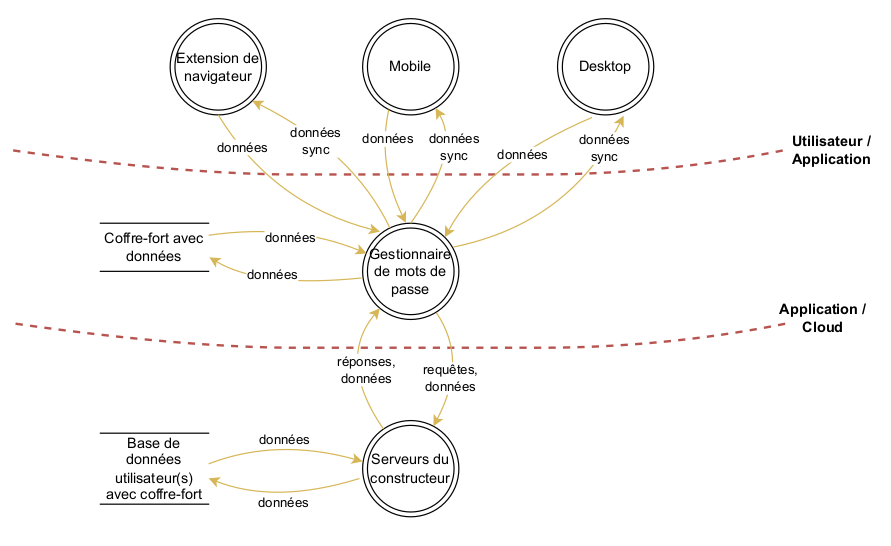
\includegraphics[width=13cm]{images/dfd_sync.png}
	\centering
	\caption{Data Flow Diagram pour les synchronisations}
\end{figure}

\subsubsection{Identification des risques}

Nous allons procéder exactement comme la section précédente, nous allons premièrement identifier les biens, menaces (avec les sources de menaces et les scénarios), les contrôles, les vulnérabilités ainsi que les conséquences sur l'entreprise afin d'établir une étude complète.

\textbf{Identification des biens}

Ci-dessous les biens présents lors du processus de sauvegarde de données dans un gestionnaire de mots de passe cloud-based.

\begin{table}[H]
	\centering
	\resizebox{\textwidth}{!}{\begin{tabular}{lll}
			\hline
			Code & Bien                                & Description                                                           \\ \hline
		A1   & Gestionnaire de mots de passe & L'application du gestionnaire de mots de passe                      \\
A2   & Coffre-fort                     & Base de données avec toutes les informations stockées                \\
			A3 & Serveurs du constructeur & Serveurs qui stockent les données des utilisateur dans le cloud \\
			\hline
	\end{tabular}}
	\caption{Biens des gestionnaires de mots de passe M3}
\end{table}
\textbf{Identification des sources de menaces}

Nous allons identifier toutes les sources de menaces possibles qui pourraient survenir dans le cadre de synchronisations de données d'un gestionnaire de mots de passe. 

\begin{table}[H]
	\centering
	\begin{tabular}{cll}
		\hline
		Code & Source de menace                & Motivations                               \\ \hline
		S1   & Hackers & Amusement, gloire, challenge, argent, ego \\
		S2   & Script kiddies                  & Curiosité, ego, argent, amusement         \\
		S3   & Concurrent                      & Espionnage, réutilisation de contenu      \\
		S4   & Cybercrime                      & Argent, destruction de données            \\
		S5   & Accident humain                 & -                                         \\
		S6   & Problèmes techniques            & -                                         \\ \hline
	\end{tabular}
	\caption{Sources de menaces des gestionnaires de mots de passe M3}
\end{table}

Ci-dessous, se trouve un tableau avec différents scénarios d'attaques. Nous utilisons le modèle STRIDE afin de définir tous les types de menaces. 

\begin{table}[H]
	\centering
	\resizebox{\textwidth}{!}{\begin{tabular}{ccclll}
			\hline
			& Code & Code du bien & Scénario de menace                                                                                                            & Type de menace                & Source de menace  \\ \hline
			1 & T1   & A1           & Phishing en imitant une page de connexion                                                                                     & \textit{Spoofing}   & S1, S2, S3, S4     \\
			2 & T1   & A1           & \begin{tabular}[c]{@{}l@{}}Attaque XSS avec les champs de connexion\\ auto-complétés\end{tabular}                             & \textit{Spoofing}     & S1, S2, S4          \\	
			3 & T3   & A1           & Clickjacking                                                                                                                            & \textit{Information Disclosure}           & S1, S2, S4  \\
			4 & T3   & A3           & \begin{tabular}[c]{@{}l@{}}Communication non chiffrée entre gestionnaire\\ de mots de passe et serveurs\end{tabular}                                                                                  & \textit{Information Disclosure}          & S1, S2, S4, S6   \\
			5 & T3   & A3, A2           & MITM (Interception de données non-chiffrées)                                                                                  & \textit{Information Disclosure}          & S1, S2, S4, S6   \\
			6 & T4   & A3           & DoS                                                                                                                           & \textit{Denial of service}           & S1, S2, S4, S6    		\\
			7 & T5   & A3           & Perte des données utilisateurs dû à un serveur down                                                                                                                           & \textit{Equipment failure}           & S5, S6   	\\
	
			8 & T3  & A3           & Vols de données non protégées sur le serveur                                                                                  & \textit{Information disclosure} & S1, S2, S4, S6          \\				
			\\\\	\hline 
			\multicolumn{6}{l}{A1 = Gestionnaire de mots de passe | A2 = Coffre-fort | A3 = Serveurs du constructeur}\\ \hline
	\end{tabular}}
	\caption{Scénarios et types d'attaques possibles sur M3}
\end{table}

\textbf{Identification des contrôles}

Il est possible de citer quelques contrôles concernant la fonctionnalité de synchronisation de données. 

Premièrement, pour la communication avec le serveurs, tous les gestionnaires de mots de passe cloud-based utilisent le protocole HTTPS afin garantir une communication chiffrée. 

Les données synchronisée sur le device de l'utilisateur sont chiffrées et peuvent être déchiffrées dès le moment où l'utilisateur a entré le bon master password lors de sa connexion au gestionnaire de mots de passe.

Finalement, pour l'auto-complétion des champs de connexion, certains s'assurent que l'utilisateur valide s'il veut vraiment remplir ce champ afin d'éviter d'entrer les données sensibles dans des pages web clonées malveillantes.

\textbf{Identification des vulnérabilités}

Pour chaque actif identifié au préalable, nous allons analyser les vulnérabilités qui pourraient être présentes. Nous allons également ajouter la sévérité de la vulnérabilité. 

\begin{table}[H]
	\centering\resizebox{\textwidth}{!}{\begin{tabular}{cll}
			\hline
			Bien                   & Vulnérabilité                                                                                                          & Sévérité de la vulnérabilité   \\ \hline
			A1 & Auto-complétion de champs sans une interaction avec l'utilisateur          & Moyen             \\
			A1                     & Utilisation de critères de correspondance faibles lors de l'auto-complétion & Moyen           \\
			A1 & Règles d'auto-complétion HTTP ne différencie pas HTTP et HTTPS                                                                                                           & Haut           \\		
							A2                & Utilisation d'algorithmes de chiffrement plus recommandés ou trop faibles   & Haut      \\	
										A3                     & Communication non chiffrée                                                                                                  & Critique                     \\	
			A3                     & Infrastructure des serveurs pas assez stable                                                                      & Haut                         \\
			A3                     & \begin{tabular}[c]{@{}l@{}}Infrastructure des serveurs du constructeur pas protégée à quelconques intrusions \\ physiques\end{tabular}                                                                     & Bas                         \\		
			\\ \\ \hline
			\multicolumn{3}{l}{A1 = Gestionnaire de mots de passe | A2 = Coffre-fort | A3 = Serveurs du constructeur}\\ \hline
	\end{tabular}}
	\caption{Vulnérabilités présentes dans les gestionnaires de mots de passe M3}
\end{table}

\textbf{Identifications des conséquences}

Pour chaque bien défini plus haut, nous allons ajouter les conséquences qu'il pourrait y avoir dans le cas d'attaques, ainsi que ce que nous souhaitons garantir.

\begin{table}[H]
	\centering
	\resizebox{\textwidth}{!}{	\begin{tabular}{lll}
			\hline
			Bien                     & Conséquences     & Garanties                                                                                             \\ \hline
					Application (A1)         & Perte de réputation et d'image      & Disponibilité, intégrité                                                                           \\
			Base de données (A2)     & Perte de réputation et d'image, perte de données        & Confidentialité, intégrité des données             \\
			Serveurs du constructeur (A3)     & Perte de réputation et d'image, perte de données        & Disponibilité, confidentialité, intégrité des données             \\\hline
	\end{tabular}}
	\caption{Conséquences des menaces sur l'entreprise}
\end{table}

\subsubsection{Analyse des risques}
Ainsi, dans cette partie, nous allons analyser l'impact des conséquences ainsi que la probabilité que chaque scénario d'attaque identifié puisse se produire. Pour cela, nous allons utiliser plusieurs notations différentes; pour les conséquences nous aurons les niveaux suivants:


\begin{table}[H]
	\centering
	\resizebox{\textwidth}{!}{\begin{tabular}{cclllll}
			\hline 
			Bien & Menace & Scénario                                                                                                                     & Impact des conséquences & Probabilité  & Niveau de risque \\ \hline
			A1   & T1           & Phishing en imitant une page de connexion                                                                                         &    Modéré            &   Possible    &     Moyen        \\
			A1   & T1           & \begin{tabular}[c]{@{}l@{}}Attaque XSS avec les champs de connexion\\ auto-complétés\end{tabular}  &    Important            &    Possible  &   Moyen          \\
			A1   & T3           & Clickjacking  &     Modéré           &  Possible    &    Moyen         \\
			A3   & T3         & \begin{tabular}[c]{@{}l@{}}Communication non chiffrée entre gestionnaire\\ de mots de passe et serveurs\end{tabular}                    &       Catastrophique         &  Peu probable    &   Moyen           \\
			A3, A2  & T3       & MITM (Interception de données non-chiffrées)                                                                                      &      Catastrophique             &    Peu probable      &      Moyen       \\
			A3  & T4         & DoS                                                                                                   &      Modéré             &   Possible   &    Moyen         \\
			A3   & T5         & Perte des données utilisateurs dû à un serveur down                                                                                   &        Catastrophique           &     Peu probable &    Moyen         \\
			
			A3   & T3          & Vols de données non protégées sur le serveur           &   Important                &  Rare    &          Moyen     \\
			\\\\ \hline 
			\multicolumn{6}{l}{A1 = Gestionnaire de mots de passe | A2 = Coffre-fort | A3 = Serveurs du constructeur }\\ 
			\multicolumn{6}{l}{T1 = Spoofing | T2 = Elevation of privileges | T3 = Information Disclosure | T4 = Denial of service | T5 = Equipment failure | T6 = Tampering}\\ 
			\hline
	\end{tabular}}
	\caption{Analyse des risques de chaque scénario de menaces sur M3}
\end{table}
\newpage
\subsection{M4 Partage}

Nous consacrons cette section à la fonctionnalité de partage de données qui est présente sur les gestionnaires de mots de passe cloud/local-based. Afin de mieux comprendre le processus, nous avons effectué un DFD qui explique comment un objet d'un utilisateur est partagé vers un autre utilisateur:

\begin{figure}[H]
	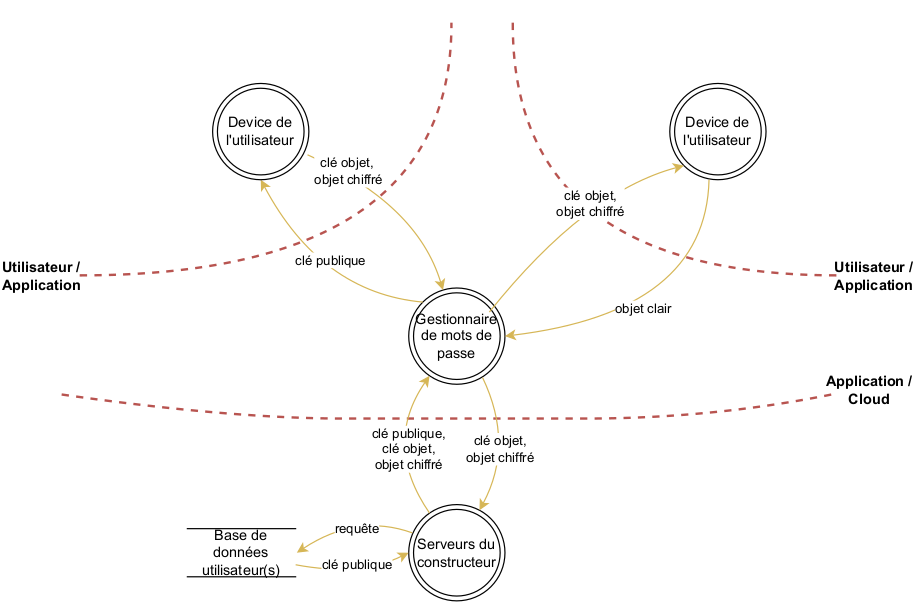
\includegraphics[width=14.5cm]{images/dfd_share.png}
	\centering
	\caption{Data Flow Diagram pour les partages de données}
\end{figure}

\subsubsection{Identification des risques}

Nous allons procéder exactement comme la section précédente, nous allons premièrement identifier les biens, menaces (avec les sources de menaces et les scénarios), les contrôles, les vulnérabilités ainsi que les conséquences sur l'entreprise afin d'établir une étude complète.

\textbf{Identification des biens}

Ci-dessous les biens présents lors du processus de partage entre deux utilisateurs.

\begin{table}[H]
	\centering
	\resizebox{\textwidth}{!}{\begin{tabular}{lll}
			\hline
			Code & Bien                                & Description                                                           \\ \hline
			A1   & Serveurs du constructeur                     & Serveurs qui stockent les données des utilisateur dans le cloud               \\
			A2 & Données partagées & Données qui sont partagées entre utilisateurs \\
			\hline
	\end{tabular}}
	\caption{Biens des gestionnaires de mots de passe M4}
\end{table}

\textbf{Identification des sources de menaces}

Nous allons identifier toutes les sources de menaces possibles qui pourraient survenir dans le cadre de partage de données d'un gestionnaire de mots de passe. 

\begin{table}[H]
	\centering
	\begin{tabular}{cll}
		\hline
		Code & Source de menace                & Motivations                               \\ \hline
		S1   & Hackers & Amusement, gloire, challenge, argent, ego \\
		S2   & Script kiddies                  & Curiosité, ego, argent, amusement         \\
		S3   & Concurrent                      & Espionnage, réutilisation de contenu      \\
		S4   & Cybercrime                      & Argent, destruction de données            \\
		S5   & Accident humain                 & -                                         \\
		S6   & Problèmes techniques            & -                                         \\ \hline
	\end{tabular}
	\caption{Sources de menaces des gestionnaires de mots de passe M4}
\end{table}

Ci-dessous, se trouve un tableau avec différents scénarios d'attaques. Nous utilisons le modèle STRIDE afin de définir tous les types de menaces. 
\begin{table}[H]
	\centering
	\resizebox{\textwidth}{!}{\begin{tabular}{ccclll}
			\hline
			& Code & Code du bien & Scénario de menace                                                                                                            & Type de menace                & Source de menace  \\ \hline
			1 & T3   & A1           & \begin{tabular}[c]{@{}l@{}}Communication non chiffrée entre gestionnaire\\ de mots de passe et serveurs\end{tabular}                                                                                  & \textit{Information Disclosure}          & S1, S2, S4, S6   \\
			2 & T3   & A1           & MITM (Interception de données non-chiffrées)                                                                                  & \textit{Information Disclosure}          & S1, S2, S4, S6   \\
			3 & T1 & A1 & Utilisateur auquel on partage des données n'est pas le bon & \textit{Spoofing} & S1, S2, S4, S6 \\
			4 & T3 & A2 & Donnée partagée non-chiffrée sur les serveurs du constructeur & \textit{Information Disclosure} & S1, S2, S4, S6 \\
			\\\\	\hline 
			\multicolumn{6}{l}{A1 = Serveurs du constructeur | A2 = Données partagées}\\ \hline
	\end{tabular}}
	\caption{Scénarios et types d'attaques possibles sur M4}
\end{table}

\textbf{Identification des contrôles}

Au niveau des contrôles effectuées lors du partage de données entre utilisateurs, il en existe quelques-uns.

Nous n'allons pas citer les contrôles que nous avons déjà pu expliquer dans les autres parties à propos de la communication des serveurs et de l'architecture \textit{Zero-knowledge}, néanmoins nous pouvons ajouter qu'ils s'assurent que même les données à partager sont chiffrées sur les serveurs et que la clé pour chiffrer l'objet est bien chiffrée avec la clé publique de l'utilisateur.

Les serveurs du constructeur contrôlent également que l'utilisateur a qui on demande sa clé publique est vraiment le bon afin d'éviter que des attaquants se fassent passer pour quelqu'un d'autre. Sur certains gestionnaires de mots de passe, ils s'assurent que la clé corresponde à l'e-mail adresse de l'utilisateur (cependant l'identité de la personne n'est pas contrôlée). 

\textbf{Identification des vulnérabilités}

Pour chaque actif identifié au préalable, nous allons analyser les vulnérabilités qui pourraient être présentes. Nous allons également ajouter la sévérité de la vulnérabilité. 

\begin{table}[H]
	\centering
	\resizebox{\textwidth}{!}{\begin{tabular}{cll}
			\hline
			Bien                   & Vulnérabilité                                                                                                          & Sévérité de la vulnérabilité   \\ \hline
			A1                     & Communication non chiffrée                                                                                                  & Critique                     \\
			A1                     & Manque de chiffrement lorsque les données sont envoyées sur les serveurs	& Critique \\
			A1 & Manque de contrôle au niveau de l'identité de la personne & Moyen \\
			A2 & Non chiffrement de données	sensibles & Critique \\
			\\ \\ \hline
			\multicolumn{3}{l}{A1 = Serveurs du constructeur | A2 = Données partagées}\\ \hline
	\end{tabular}}
	\caption{Vulnérabilités présentes dans les gestionnaires de mots de passe M4}
\end{table}

\textbf{Identifications des conséquences}

Pour chaque bien défini plus haut, nous allons ajouter les conséquences qu'il pourrait y avoir dans le cas d'attaques, ainsi que ce que nous souhaitons garantir.

\begin{table}[H]
	\centering
	\resizebox{\textwidth}{!}{	\begin{tabular}{lll}
			\hline
			Bien                     & Conséquences     & Garanties                                                                                             \\ \hline
			Serveurs du constructeur (A1)         & Perte de réputation et d'image, pertes de données      & Disponibilité, intégrité, confidentialité                                                                           \\
			Données partagées (A2)     & Perte de réputation et d'image, perte de données        & Confidentialité, intégrité des données             \\ \hline
	\end{tabular}}
	\caption{Conséquences des menaces sur l'entreprise}
\end{table}

\subsubsection{Analyse des risques}
Ainsi, dans cette partie, nous allons analyser l'impact des conséquences ainsi que la probabilité que chaque scénario d'attaque identifié puisse se produire. Pour cela, nous allons utiliser plusieurs notations différentes; pour les conséquences nous aurons les niveaux suivants:

\begin{table}[H]
	\centering
	\resizebox{\textwidth}{!}{\begin{tabular}{cclllll}
			\hline 
			Bien & Menace & Scénario                                                                                                                     & Impact des conséquences & Probabilité  & Niveau de risque \\ \hline
			A1   & T3           & \begin{tabular}[c]{@{}l@{}}Communication non chiffrée entre gestionnaire\\ de mots de passe et serveurs\end{tabular}                                                                          &     Catastrophique           &  Peu probable     &     Moyen        \\
			A1   & T3           & MITM (Interception de données non-chiffrées) &   Catastrophique            &  Peu probable    &       Moyen      \\
			A1   & T1        & Utilisateur auquel on partage des données n'est pas le bon              &       Important            &  Probable   &     Haut         \\
			A2   & T3        & Donnée partagée non-chiffrée sur les serveurs du constructeur                                                                                      &       Important            &    Peu probable      &       Moyen      \\
			\\\\ \hline 
			\multicolumn{6}{l}{A1 = Serveurs du constructeur | A2 = Données partagées }\\ 
			\multicolumn{6}{l}{T1 = Spoofing | T2 = Elevation of privileges | T3 = Information Disclosure | T4 = Denial of service | T5 = Equipment failure | T6 = Tampering}\\ 
			\hline
	\end{tabular}}
	\caption{Analyse des risques de chaque scénario de menaces sur M4}
\end{table}

\newpage

\subsection{M5 Application bas-niveau}

La dernière partie de cette analyse de menaces concerne la sécurité des gestionnaires de mots de passe et de tous ses composants, donc tout le bas-niveau. Cela inclut le stockage des données sensibles (clés, coffre-fort, master password) en mémoire RAM ainsi que sur le disque (fichiers de sauvegardes). Puis, nous aborderons les processus de chiffrement et génération des clés.

Ci-dessous un schéma représentant l'architecture bas-niveau des applications.

\begin{figure}[H]
	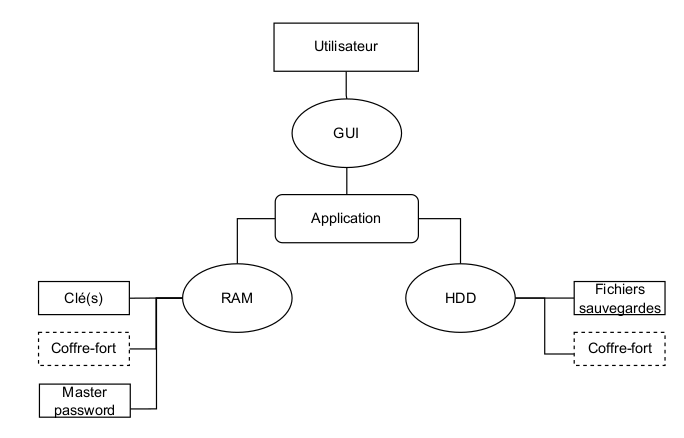
\includegraphics[width=14.5cm]{images/dfd_low.png}
	\centering
	\caption{Schéma bas-niveau des gestionnaires de mots de passe}
\end{figure}

\subsubsection{Identification des risques}

Nous allons procéder exactement comme la section précédente, nous allons premièrement identifier les biens, menaces (avec les sources de menaces et les scénarios), les contrôles, les vulnérabilités ainsi que les conséquences sur l'entreprise afin d'établir une étude complète.

\textbf{Identification des biens}

Ci-dessous les biens concernant la sécurité bas-niveau des gestionnaires de mots de passe.

\begin{table}[H]
	\centering
	\resizebox{\textwidth}{!}{\begin{tabular}{lll}
			\hline
			Code & Bien                                & Description                                                 \\ \hline
			A1   & Coffre-fort                    &   Base de données avec toutes les informations stockées             \\
			A2 & Master password & Mot de passe principal afin de déchiffrer le coffre-fort \\
			A3 & Clés & Clé(s) de chiffrement et privée(s) de l'utilisateur  \\			
			\hline
	\end{tabular}}
	\caption{Biens des gestionnaires de mots de passe M5}
\end{table}
\textbf{Identification des sources de menaces}

Nous allons identifier toutes les sources de menaces possibles qui pourraient survenir au niveau bas-niveau de l'application. 

\begin{table}[H]
	\centering
	\begin{tabular}{cll}
		\hline
		Code & Source de menace                & Motivations                               \\ \hline
		S1   & Hackers & Amusement, gloire, challenge, argent, ego \\
		S2   & Script kiddies                  & Curiosité, ego, argent, amusement         \\
		S3   & Concurrent                      & Espionnage, réutilisation de contenu      \\
		S4   & Cybercrime                      & Argent, destruction de données            \\
		S5   & Accident humain                 & -                                         \\
		S6   & Problèmes techniques            & -                                         \\ \hline
	\end{tabular}
	\caption{Sources de menaces des gestionnaires de mots de passe M5}
\end{table}

Ci-dessous, se trouve un tableau avec différents scénarios d'attaques. Nous utilisons le modèle STRIDE afin de définir tous les types de menaces. 
\begin{table}[H]
	\centering
	\resizebox{\textwidth}{!}{\begin{tabular}{ccclll}
			\hline
			& Code & Code du bien & Scénario de menace                                                                                                            & Type de menace                & Source de menace  \\ \hline
			1 & T3   & A1           & Récupération de données sensibles en clair sur le disque                                                                      & \textit{Information disclosure}      & S1, S2, S4 \\
			2 & T3   & A1           & \begin{tabular}[c]{@{}l@{}}Récupération du coffre-fort et déchiffrement\\ dû à un algorithme trop simple\end{tabular}  & \textit{Information disclosure}    & S1, S2, S4    \\
			3 & T3   & A1, A2, A3           & Récupération de données sensibles en mémoire                                                                                  & \textit{Information Disclosure}    & S1, S2, S4     \\
			4 & T3   & A3           & Récupération de la clé de chiffrement en mémoire                                                                              & \textit{Information Disclosure}    & S1, S2, S4 \\
			5 & T3   & A3           & Brute-force de clé                                                                                                            & \textit{Information Disclosure}    & S1, S2, S4    \\                                                     
			
			\\\\	\hline 
			\multicolumn{6}{l}{A1 = Coffre-fort | A2 = Master password | A3 = Clés}\\ \hline
	\end{tabular}}
	\caption{Scénarios et types d'attaques possibles sur M5}
\end{table}

\textbf{Identification des contrôles}

Le contrôle qui est présent sur toutes les applications est que chaque utilisateur possède une clé de chiffrement différente, qui est dérivée avec son master password. Même si ce dernier est le même, la clé ne sera pas pareille dû au salt qui est soit aléatoire soit le username, qui est unique. Les algorithmes choisis sont forts (voir \ref{crypto}) et sont recommandés pour la dérivation des clés. Ainsi, la clé est protégée contre le brute-force ou les attaques par dictionnaire. Néanmoins, il est quand même important d'avoir un master password fort\footnote{Ce qu'on considère un mot de passe fort; au moins une majuscule, une minuscule, un chiffre et 11 caractères}, ce qui n'est pas demandé dans tous les gestionnaires de mots de passe lors de l'inscription de l'utilisateur.

Pour le chiffrement des données, les gestionnaires de mots de passe utilisent AES-256. L'algorithme est également encore recommandé en 2022.

Au niveau de la protection mémoire, certains proposent une protection des données sensibles dans le processus (avec DPAPI ou Chacha20) et les données sont effacées sur le disque dès que le processus s'arrête. En se basant sur une étude\cite{iseexploit}, la mémoire est en général bien protégée lorsque le gestionnaire dans l'état \textit{Not Running}, cependant dès le moment où le gestionnaire est dans l'état \textit{Unlock} ou \textit{Locked}, les secrets et le master password sont plus exposés. 

\textbf{Identification des vulnérabilités}

Pour chaque actif identifié au préalable, nous allons analyser les vulnérabilités qui pourraient être présentes. Nous allons également ajouter la sévérité de la vulnérabilité. 

\begin{table}[H]
	\centering
	\resizebox{\textwidth}{!}{\begin{tabular}{cll}
			\hline
			Bien                   & Vulnérabilité                                                                                                          & Sévérité de la vulnérabilité   \\ \hline
				A1                 & \begin{tabular}[c]{@{}l@{}}Utilisation d'algorithmes de chiffrement plus recommandés ou \\ trop faibles\end{tabular}   & Haut                       \\
				A1, A2, A3                     & Aucune protection de la mémoire du processus                                                                           & Haut         \\
				A1, A2, A3                     & Option \textit{remember me}                                                                                                   & Haut                \\
				\multicolumn{1}{c}{A1, A2, A3} & Données non nettoyées de la mémoire lors de l'arrêt du processus           & Haut                   \\	

A3                     & Dérivation des clés trop simple                                                                                        & Moyen             \\											
			\\ \\ \hline
			\multicolumn{3}{l}{A1 = Coffre-fort | A2 = Master password | A3 = Clés}\\ \hline
	\end{tabular}}
	\caption{Vulnérabilités présentes dans les gestionnaires de mots de passe M5}
\end{table}

\textbf{Identifications des conséquences}

Pour chaque bien défini plus haut, nous allons ajouter les conséquences qu'il pourrait y avoir dans le cas d'attaques, ainsi que ce que nous souhaitons garantir.

\begin{table}[H]
	\centering
	\resizebox{\textwidth}{!}{	\begin{tabular}{lll}
			\hline
			Bien                     & Conséquences     & Garanties                                                                                             \\ \hline
			Coffre-fort (A1)         & Perte de réputation et d'image, pertes de données      & Intégrité, confidentialité                                                                           \\
			Master password (A2)     & Perte de réputation et d'image, perte de données        & Confidentialité, intégrité des données             \\
			Clés (A3)     & Perte de réputation et d'image, perte de données        & Confidentialité, intégrité              \\ \hline
	\end{tabular}}
	\caption{Conséquences des menaces sur l'entreprise}
\end{table}

\subsubsection{Analyse des risques}
Ainsi, dans cette partie, nous allons analyser l'impact des conséquences ainsi que la probabilité que chaque scénario d'attaque identifié puisse se produire. Pour cela, nous allons utiliser plusieurs notations différentes; pour les conséquences nous aurons les niveaux suivants:

\begin{table}[H]
	\centering
	\resizebox{\textwidth}{!}{\begin{tabular}{cclllll}
			\hline 
			Bien & Menace & Scénario                                                                                                                     & Impact des conséquences & Probabilité  & Niveau de risque \\ \hline
			A1   & T3           & Récupération des données sensibles en clair sur le disque &     Important           &   Probable   &   Haut          \\
			A1   & T3         & \begin{tabular}[c]{@{}l@{}}Récupération du coffre-fort et déchiffrement\\ dû à un algorithme trop simple\end{tabular}             &    Important            &   Peu probable   &     Moyen         \\
			A1, A2, A3   & T3        & Récupération de données sensibles en mémoire                                                                            &     Important              &     Probable     &   Haut          \\
			A3  & T3         & Récupération de la clé de chiffrement en mémoire                                                                           &    Important               &   Probable   &       Haut      \\
			A3   & T3         & Brute-force de clé                                                                                  &     Important              &  Rare    &    Moyen         \\
			
			\\\\ \hline 
			\multicolumn{6}{l}{A1 = Coffre-fort | A2 = Master password | A3 = Clés}\\ 
			\multicolumn{6}{l}{T1 = Spoofing | T2 = Elevation of privileges | T3 = Information Disclosure | T4 = Denial of service | T5 = Equipment failure | T6 = Tampering}\\ 
			\hline
	\end{tabular}}
	\caption{Analyse des risques de chaque scénario de menace sur M5}
\end{table}

\subsection{Évaluation des risques}

Cette étape sert à évaluer si les risques sont acceptables ou s'ils ont besoin d'un traitement supplémentaires, c'est-à-dire une mitigation. Nous avons défini à l'étape précédente le niveau de risque de chaque scénario de menace. En résumé, nous avons:

\begin{itemize}
	\item Bas: 2
	\item Moyen: 17
	\item Haut: 6
\end{itemize} 

Ainsi, nous pouvons définir que les tous les scénarios de menaces ayant un niveau de risque bas peuvent être acceptés par l'entreprise, néanmoins ces derniers ne doivent pas être oubliés et mis de côté. Pour les niveaux de risques moyen et haut, il est nécessaire d'appliquer une mitigation et de surveiller les menaces. 

\subsection{Traitement des risques}
Dans cette section, nous allons définir les contre-mesures à entreprendre afin d'éviter au maximum les menaces que nous avons identifié plus haut. Comme précisé dans le paragraphe de l'identification des contrôles, beaucoup de choses sont déjà mises en place par les constructeurs et sont efficaces contre les attaques. Néanmoins, nous pouvons ajouter quelques contre-mesures qui ne sont pas ou peu effectuées par les quelques candidats que nous avons sélectionnés au préalable. Ainsi, nous allons sélectionner les risques qui ont été qualifiés comme moyen ou haut et nous allons proposer des contre-mesures possibles.

	\begin{table}[H]
	\centering
	\resizebox{\textwidth}{!}{\begin{tabular}{l|l}
		\hline
		\textbf{Menace}                                    & \textbf{Contre-mesures }                                                                                                                                                                                                                                                                                                          \\ \hline
		Master password faible                    & \begin{tabular}[c]{@{}l@{}}- Ajouter des contrôles lors de l'inscription de l'utilisateur en lui demandant un mot de passe fort\\ - Proposer un master password fort généré aléatoirement par l'application\end{tabular}                                                                                                 \\ \hline
		Temps de session trop long                & - Ajouter un temps d'expiration de session et verrouiller le gestionnaire après ce temps                                                                                                                                                                                                                                 \\ \hline
		Presse-papier non nettoyé                 & - Après un temps court, nettoyer le presse-papier de l'utilisateur                                                                                                                                                                                                                                                       \\ \hline
		Brute-force               & 
		\begin{tabular}[c]{@{}l@{}} - Ajouter un nombre d'essais maximum \\ - Ajouter une politique de master password forte\end{tabular}                                                                               \\ \hline
		Phishing en clonant une page de connexion & \begin{tabular}[c]{@{}l@{}}- Appliquer un meilleur critère de match lors de l'auto-complétion des champs\\ de connexion\\ - Demander à l'utilisateur de valider l'auto-complétion         \\ - Sensibilisation auprès des utilisateurs  \end{tabular}                                                                                                                \\ \hline
		Clickjacking                              & - Bloquer l'utilisation de Javascript à l'aide d'API sécurisées                                                                                                                                                                                                                                                          \\ \hline
		Communication non-chiffrée                & \begin{tabular}[c]{@{}l@{}}- Ajouter HTTPS pour la communication avec le serveur\\ - Éviter d'envoyer le master password ou des clés de chiffrement ou\\ privée au serveur\\ - Chiffrer toutes les données avant de les envoyer dans le cloud\end{tabular}                                                               \\ \hline
		Dérivation des clés trop simple           & \begin{tabular}[c]{@{}l@{}}- Utiliser un algorithme recommandé et fort (PBKDF2-SHA2 par exemple)\\ - Une clé de chiffrement unique par utilisateur pour éviter le brute force\end{tabular}                                                                                                                               \\ \hline
		Perte de données                          & \begin{tabular}[c]{@{}l@{}}- Si cloud-based / browser-based, effectuer des backups sur les serveurs chaque\\ nuit\\ - Mettre à disposition la fonctionnalité de backup pour les particuliers pour les \\ faire en local\\ - Exportation des données CSV et les stocker dans un endroit chiffrer et sécurisé\end{tabular} \\ \hline
		Manque de protection dans la mémoire      & \begin{tabular}[c]{@{}l@{}}- Nettoyage de mémoire lorsque le gestionnaire est dans l'état locked\\ - Protection des données sensible avec des APIs pour limiter l'exposition\\ de secrets\end{tabular}                                                                                                                   \\ \hline
		\multicolumn{1}{l|}{Option remember me}  & \multicolumn{1}{l}{- Désactivation de mode offline avec les gestionnaires cloud-based et browser-based}                                                                                                                                                                                                                 \\ \hline
		Manque de protection du disque & - Utiliser un chiffrement du disque entier \\ \hline
	\end{tabular}}
\caption{Contre-mesures possibles pour les gestionnaires}
\end{table}

\section{Exigences sécuritaires à respecter} 
Dans cette dernière section de l'analyse de menaces, nous allons établir une liste d'exigences sécuritaires que les gestionnaires de mots de passe doivent respecter afin de se définir sécurisé et afin de protéger les données sensibles au maximum. Nous allons premièrement identifier toutes les exigences générales puis nous allons les définir plus en détails afin d'expliquer ce que nous souhaitons garantir.
%\multirow{5}{*}{\STAB{\rotatebox[origin=c]{90}{\textbf{Chiffrement}}}}
Pour les identifier, nous allons nous référencer à notre analyse de menaces puis nous allons également nous baser sur le standard de OWASP \textit{Application Security Verification Standard}\cite{ASVS}. 
\begin{landscape}
	\centering
	\fontsize{8}{11}\selectfont
\begin{longtable}[H]{c|l|l}
			\hline
			\multicolumn{1}{c|}{\textbf{Type}} & \multicolumn{1}{c|}{\textbf{Description de l'exigence}} & \multicolumn{1}{c}{\textbf{Commentaire}}  \\ \hline
			\multirow{5}{*}{\textbf{Chiffrement}}      & \begin{tabular}[c]{@{}l@{}}Le coffre-fort de l'utilisateur doit impérativement être chiffré avec\\ un algorithme ainsi qu'une taille de clé qui sont recommandés\end{tabular}         & \begin{tabular}[c]{@{}l@{}}Nous pouvons nous baser sur les recommandations \\ du report de ECRYPT\cite{ecrypt}. Au mieux, l'algorithme \\ devrait être encore recommandé pour une utilisation \\  future.\end{tabular} \\ \cline{2-3} 
			& \begin{tabular}[c]{@{}l@{}}Le chiffrement doit être end-to-end pour assurer la protection de\\ données lors du transport dans le cloud\end{tabular}                                   & \begin{tabular}[c]{@{}l@{}}Concerne les gestionnaires qui fonctionnent avec le\\ cloud et font de la synchronisations de données\end{tabular}                                                                                       \\ \cline{2-3} 
			& Le chiffrement doit être fait côté client, donc en local                                                                                                                              & \begin{tabular}[c]{@{}l@{}}Afin d'éviter que des données claires soient stockés sur\\ les serveurs\end{tabular}                                                                                                                     \\ \cline{2-3} 
			& L'architecture Zero-knowledge doit être respectée                                                                                                                                     & Cette exigence est identique à la précédente                                                                                                                                                                                        \\ \cline{2-3} 
			& \begin{tabular}[c]{@{}l@{}}La communication entre l'utilisateur et les serveurs doit être \\ chiffrée avec un algorithme recommandé\end{tabular}                                      & HTTPS est la meilleure solution de chiffrement                                                                                                                                                                                      \\ \hline
			\multirow{5}{*}{\textbf{Clés de chiffrement}} & \begin{tabular}[c]{@{}l@{}}La dérivation de clé.s doit se baser sur des algorithmes \\ Password-Based Key Derivation et doit être recommandé\end{tabular}                             & \begin{tabular}[c]{@{}l@{}}Les plus courants sont Argon2 et PBKDF2 (associé à \\ une fonction de hash)\end{tabular}                                                                                                                 \\ \cline{2-3} 
			& Le salt doit être unique                                                                                                                                                              & \begin{tabular}[c]{@{}l@{}}Si on utilise le username ou l'adresse e-mail, il faut\\ absolument s'assurer que ce dernier soit unique lors de\\ l'inscription de l'utilisateur\end{tabular}                                           \\ \cline{2-3} 
			& Le salt doit être aléatoire (si on n'utilise pas le username)                                                                                                                         & \begin{tabular}[c]{@{}l@{}}Utiliser un pseudo-nombre généré aléatoirement \\ pour s'assurer qu'il soit correctement aléatoire\end{tabular}                                                                                          \\ \cline{2-3} 
			& \begin{tabular}[c]{@{}l@{}}Les clés et la salt doivent être stockés localement dans la mémoire\\ du processus\end{tabular}                                                            &                                                                                                                                                                                                                                     \\ \cline{2-3} 
			& \begin{tabular}[c]{@{}l@{}}Les clés de chiffrement ne doivent jamais être envoyées \\ aux serveurs et rester en local\end{tabular}                                                    & Pour les gestionnaires qui utilisent le cloud                                                                                                                                                                                       \\ \hline
			\multirow{3}{*}{\textbf{Authentification}}   & \begin{tabular}[c]{@{}l@{}}Authentifier les données avec un schéma sûr, comme Encrypt-\\ then-MAC\end{tabular}                                                                        & \begin{tabular}[c]{@{}l@{}}Nécessaire pour les gestionnaires qui ne \\ fonctionnent qu'en local\end{tabular}                                                                                                                        \\ \cline{2-3} 
			& Authentifier les utilisateurs auprès des serveurs du constrtucteur                                                                                                                    & \begin{tabular}[c]{@{}l@{}}Pour les gestionnaires qui fonctionnent \\ également avec le cloud\end{tabular}                                                                                                                          \\ \cline{2-3} 
			& \begin{tabular}[c]{@{}l@{}}Hash d'authentification stocké dans la base de données des \\ serveurs doit être chiffré\end{tabular}                                                      & \begin{tabular}[c]{@{}l@{}}Hash utilisé pour le comparer avec celui que le client\\ envoie afin d'approuver l'authentification\end{tabular}                                                                                         \\ \hline
			\multirow{5}{*}{\textbf{Master password}}     & \begin{tabular}[c]{@{}l@{}}Le master password doit respecter des critères lors de\\ l'inscription de l'utilisateur\end{tabular}                                                       & \begin{tabular}[c]{@{}l@{}}Pour que le master password soit fort et qu'on évite au\\ maximum des attaques sur mots de passe\end{tabular}                                                                                            \\ \cline{2-3} 
			& Le master password ne devrait jamais être stocké en mémoire                                                                                                                           & \begin{tabular}[c]{@{}l@{}}À moins que des précautions de protection de mémoire \\ aient été prises et qu'on ne puisse pas le voir en clair\end{tabular}                                                                            \\ \cline{2-3} 
			& La fonctionnalité Remember me est fortement déconseillée                                                                                                                              & \begin{tabular}[c]{@{}l@{}}Dû au fait que le master password puisse être stocké en\\ mémoire\end{tabular}                                                                                                                           \\ \cline{2-3} 
			& \begin{tabular}[c]{@{}l@{}}Demander obligatoirement le 2FA ou MFA à l'utilisateur lors de\\ son inscription\end{tabular}                                                              & Cela permet d'ajouter une couche sécuritaire                                                                                                                                                                                        \\ \cline{2-3} 
			& \begin{tabular}[c]{@{}l@{}}Le master password devrait rester localement et ne devrait jamais\\ être transmis aux serveurs\end{tabular}                                                & Pour les gestionnaires qui fonctionnent avec le cloud                                                                                                                                                                               \\ \hline
			\textbf{Session}                              & Un temps de session doit être ajouté obligatoirement                                                                                                                                  & \begin{tabular}[c]{@{}l@{}}Le gestionnaire se place dans un état Locked après\\ ce temps\end{tabular}                                                                                                                               \\ \hline
			\multirow{4}{*}{\textbf{Mémoire}}             & \begin{tabular}[c]{@{}l@{}}Dans l'état Not Running, aucune donnée qui puisse faire\\ compromettre la base de données sur le disque ne doit être \\ stockée sur le disque\end{tabular} & \begin{tabular}[c]{@{}l@{}}Par exemple, le master password ou une clé\\ de chiffrement dans un fichier de configuration\end{tabular}                                                                                                \\ \cline{2-3} 
			& \begin{tabular}[c]{@{}l@{}}Dans l'état Unlocked, il devrait pas être possible d'extraire le\\ master password de la mémoire\end{tabular}                                              &                                                                                                                                                                                                                                     \\ \cline{2-3} 
			& \begin{tabular}[c]{@{}l@{}}Dans l'état Unlocked, il ne devrait pas être possible d'extraire de\\ la mémoire des éléments déchiffrés avec lesquels on n'a pas interagi\end{tabular}    & \begin{tabular}[c]{@{}l@{}}Une interaction peut être afficher, copier ou encore\\ l'accès aux mots de passe\end{tabular}                                                                                                            \\ \cline{2-3} 
			& \begin{tabular}[c]{@{}l@{}}Dans l'état Locked, il ne devrait pas être possible d'extraire\\ n'importe quelle donnée sensible\end{tabular}                                             & \begin{tabular}[c]{@{}l@{}}Toutes les données doivent être effacées de la \\ mémoire\end{tabular}                                                                                                                                   \\ \hline
			\multirow{4}{*}{\textbf{Partage de données}}  & \begin{tabular}[c]{@{}l@{}}Les clés privées ne devraient être accessibles qu'aux utilisateurs\\ concernés\end{tabular}                                                                &                                                                                                                                                                                                                                     \\ \cline{2-3} 
			& \begin{tabular}[c]{@{}l@{}}Les clés privées doivent rester en local et ne jamais être envoyé\\ aux serveurs\end{tabular}                                                              &                                                                                                                                                                                                                                     \\ \cline{2-3} 
			& Les clés publiques et les identités liées doivent être vérifiées                                                                                                                      & \begin{tabular}[c]{@{}l@{}}Afin de s'assurer que l'utilisateur a qui on demande\\ sa clé est le bon\end{tabular}                                                                                                                    \\ \cline{2-3} 
			& \begin{tabular}[c]{@{}l@{}}L'élément a partager et sa clé de chiffrement doivent être chiffrés\\ localement\end{tabular}                                                              &                                                                                                                                                                                                                                     \\ \hline
			\textbf{Backup}                               & Les sauvegardes stockées sur les serveurs doivent être chiffrées                                                                                                                      &                                                                                                                                                                                                                                     \\ \hline
			\textbf{Presse-papier}                        & \begin{tabular}[c]{@{}l@{}}Le presse-papier doit être nettoyé après un court instant (10-40s),\\ l'historique du presse-papier doit également être nettoyé\end{tabular}               & Pour éviter le sniffing de presse-papier                                                                                                                                                                                            \\ \hline
			\multirow{5}{*}{\textbf{Attaques web-based}   }                & \begin{tabular}[c]{@{}l@{}}Pour l'auto-complétion des champs, il est nécessaire de demander\\ l'autorisation à l'utilisateur pour remplir le champs\end{tabular}                      & Cela peut faire évitter des attaques de phishing                                                                                                                                                                                    \\ \cline{2-3} 
			& \begin{tabular}[c]{@{}l@{}}Les critères de matching pour les URLs lors de l'auto-complétion\\ doivent être stricts\end{tabular}                                                       &                                                                                                                                                                                                                                     \\ \cline{2-3} 
			& Éviter d'ignorer les sous-domaines de l'URL                                                                                                                                           & \begin{tabular}[c]{@{}l@{}}Afin de s'assurer qu'il n'est pas possible de voler les\\ identifiants du domaine parent\end{tabular}                                                                                                    \\ \cline{2-3} 
			& \begin{tabular}[c]{@{}l@{}}Il faudrait faire la différence entre HTTP et HTTPS lors du remplissage\\ automatique des champs\end{tabular}                                              & \begin{tabular}[c]{@{}l@{}}Pour éviter une attaque MITM et de remplir une page\\ clônée HTTP d'un  site initalement HTTPS\end{tabular}                                                                                              \\ \cline{2-3} 
			& Il faut bloquer l'exécution Javascript   \\\hline
						\caption{Exigences sécuritaires}  
                                                                                                                                         
\end{longtable}

\end{landscape}

% +---------------------------------------------------------------+
% | Author :    Noémie Plancherel, HEIG-VD
% | Date :      20.09.2022
% +---------------------------------------------------------------+

\chapter{Sélection des candidats}
\label{ch:selection}
Dans ce chapitre, nous allons faire la sélection des gestionnaires de mots de passe que nous analyserons dans le
chapitre suivant. Nous définirons les critères des sélections afin de correctement les choisir, puis nous ferons
notre choix en fonction des candidats sélectionnés. Afin d'avoir une bonne vue d'ensemble sur les fonctionnalités et
la sécurité de chaque application, nous allons reprendre les 9 gestionnaires analysés dans les chapitres précédents.

\section{Critères de sélection}

Cette section va ainsi présenter les critères de sélections pour les candidats avec lesquels on fera une analyse
sécuritaire détaillée.

\textbf{Open-source} - un critère assez important car un gestionnaire de mots de passe open-source pourrait être plus
sûr qu'un gestionnaire closed-source dû au fait qu'importe quel utilisateur peut auditer le code source
indépendamment et peut reporter des failles aux constructeurs. Les applications closed-source comptent à 100\% sur
l'équipe de développement et pourrait faire face à plus d'attaques.

\textbf{Types} - nous allons sélectionner des gestionnaires des 3 types différents afin d'avoir un éventail complet
de gestionnaires de mots de passe existants. Pour faire un rappel, les différents types sont: cloud-based,
local-based et browser-based.

\textbf{Gratuit} - il est bien de prendre en compte ce critère afin d'analyser si un gestionnaire proposant des
fonctionnalités gratuites est plus faible qu'un gestionnaire complètement payant. De plus, il pourrait être
intéressant de comparer la sécurité d'un application qui propose des fonctionnalités gratuites et payantes.

\textbf{Nombre d'utilisateurs} - il est intéressant d'ajouter le critère de la popularité afin de se rendre compte
de l'impact de quelconques vulnérabilités présentes sur l'application et de constater malgré une grande
popularité, s'il y a l'existence de failles non-corrigées ou non-prises en compte.

\textbf{Partage de données} - cette fonctionnalité est assez critique, dû au fait que des données sont partagées
entre plusieurs utilisateurs, il est impératif que les données soient uniquement accessibles par les bonnes personnes
de confiance. Ainsi, il serait intéressant de sélectionner au moins un candidat qui propose cette fonctionnalité pour
évaluer la sécurité.

\textbf{Choix cryptographiques} - ce critère concerne les choix cryptographiques utilisés pour le chiffrement des
données par exemple, ou la dérivation des clés. Il sera important d'évaluer si ces choix sont suffisant. Ainsi, nous
allons sélectionner des candidats qui ont effectuer des choix cryptographiques différents.

\textbf{Plateforme supportée} - l'analyse sécuritaire se fera dans un premier temps sur un ordinateur avec Windows
11, donc les applications doivent être disponibles pour cet OS. La raison pour laquelle nous faisons ce choix est que c'est un des OS les plus populaires sur le marché.

\textbf{Failles connues} - pour quelques gestionnaires de mots de passe, des vulnérabilités ont été découvertes. Pour
certaines, des corrections ont été faites aux applications mais certaines n'ont pas été corrigée malgré un report
vers les constructeurs des gestionnaires. Ainsi, ceci est un aspect important à prendre en compte afin de constater
si les failles ont été corrigées après leurs découvertes.

\section{Choix}
Afin d'avoir une bonne vue d'ensemble sur tous les candidats et de faire une sélection pertinente, nous allons
établir un tableau récapitulatif. Lors du choix, nous allons tenter de couvrir tous les critères proposés avant, afin
de faire une analyse complète et diverse sur tout ce qui existe sur le marché actuellement.

Nous allons donc choisir X candidats pour avoir une bonne vue d'ensemble sur tout ce qui existe.

\begin{figure}[H]
	\centering
	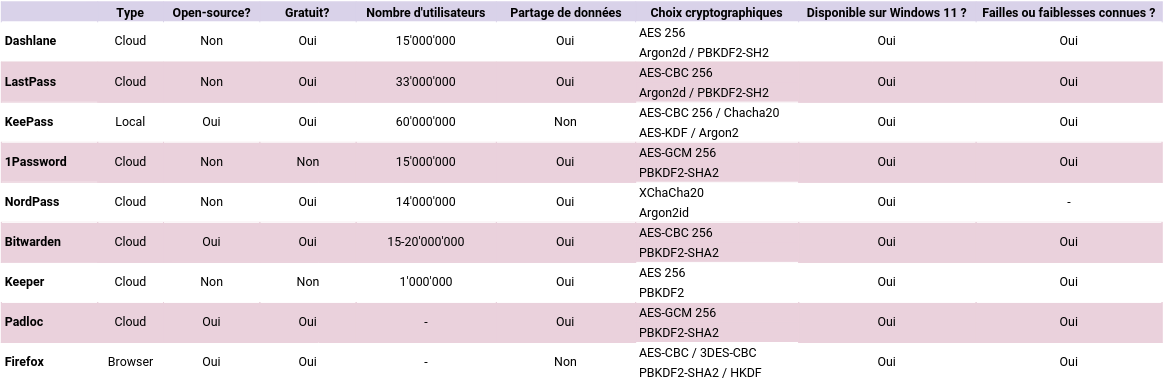
\includegraphics[scale=0.5, angle=90]{images/selection_choix.png}
	\caption{Comparatif des candidats pour la sélection}
\end{figure}

Ainsi, nous allons sélectionner:
\begin{itemize}
	\item LastPass
	\item KeePass
	\item Firefox
	\item 1Password
\end{itemize}

Chaque chapitre dédié aux gestionnaires de mots de passe sélectionnés se basera sur les exigences sécuritaires que nous avons définis au chapitre précédent et sur les vulnérabilités et faiblesses déjà connues. 

À chaque début de chapitre, nous établirons les critères d'évaluation de la sécurité de l'application. Les critères seront à chaque fois différents en fonction du type ou des fonctionnalités proposées. 




% +---------------------------------------------------------------+
% | Author :    Noémie Plancherel, HEIG-VD
% | Date :      16.10.2022
% +---------------------------------------------------------------+

\chapter{KeePass}
\label{ch:keepass}

Ce chapitre sera dédié à l'analyse sécuritaire de l'application KeePass. Nous allons utiliser l'application desktop sur Windows 11. KeePass fonctionne entièrement en local et aucune donnée ne transitent sur le cloud. 

Nous voulons préciser que KeePass est open-source, ce qui va nous permettre d'analyser le code en cas de vulnérabilités trouvées. De  plus, cela nous permettra de proposer une correction du code afin de contribuer au gestionnaire de mots de passe.

\section{Environnement}

\begin{table}[H]
	\centering
	\begin{tabular}{ll}
		\hline
		Logiciel           & Version        \\ \hline
		Windows 11         & 10.0.22621     \\
		KeePass & 2.52       \\ \hline
	\end{tabular}
	\caption{Environnement utilisé pour KeePass}
\end{table}

Pour cette analyse, nous allons utiliser KeePass sans plugin supplémentaire, afin d'analyser l'application basique sans aucun ajout. Nous procédons de cette manière-ci car il existe beaucoup de plugins différents qui permettent d'ajouter des fonctionnalités différentes, comme des backups, une couche sécuritaire supplémentaire, de l'export, etc\footnote{\href{https://keepass.info/plugins.html}{https://keepass.info/plugins.html}}. Cependant, chaque plugin est développé par des personnes externes à KeePass, ainsi il est préférable de ne pas les inclure dans le rapport.

De plus, KeePass propose deux versions de son application, une 1.x et une 2.x. La première propose beaucoup moins de fonctionnalités et est moins flexible que la deuxième, c'est pour cela que nous nous basons sur la deuxième.
\section{Critères d'analyse}

L'établissement des critères d'analyse se basent sur l'analyse de menaces effectuée plus tôt dans le travail et sur les failles connues de KeePass afin qu'on puisse se baser dessus.

\begin{itemize}
	\item Master password
	\item Choix cryptographiques
	\begin{itemize}
		\item Chiffrement
		\item Dérivation des clés
		\item Authentification
	\end{itemize}
	\item Fonctionnalités proposées
	\begin{itemize}
		\item Génération de mots de passe
		\item Presse-papier
	\end{itemize}
	\item Stockage
	\item Mémoire
\end{itemize}

\section{Master password}

Quand l'utilisateur créée sa nouvelle base de données, où toutes les données du coffre-fort seront stockées dessus, KeePass demande de fournir un master password qui permettra d'y dériver la master de key et de chiffrer le coffre-fort. 

Il n'y a pas de critères exigés par KeePass lors de la spécification, ainsi l'utilisateur pourrait ajouter un seul caractère et le master password serait validé. Néanmoins, KeePass indique qu'il s'agit d'un mot de passe faible, ce qui pourrait permettre d'éviter des master password trop faibles qui permettrait d'effectuer une attaque de brute-force:

\begin{figure}[H]
	\centering
	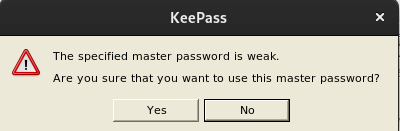
\includegraphics[width=8cm]{images/kp_weak.png}
	\caption{Avertissement de master password faible de KeePass}
\end{figure}

Le gestionnaire indique également la qualité du mot de passe en indiquant le nombre de bits d'entropie et la force du mot de passe. 

Il existe également des "options d'expert" qui permettent d'ajouter deux facteurs supplémentaires lors de la connexion. L'utilisateur peut fournir un \textit{key file} qui est un fichier qui contient une clé. Il est possible d'ajouter le compte utilisateur Windows (si on est sur cette OS), ce qui permet de faire la base de données dépendante à l'utilisateur connecté. De ce fait, il sera uniquement possible d'ouvrir le coffre-fort si on est connecté avec cet utilisateur. 

Pour chaque facteur ajouté, KeePass avertit \textbf{explicitement} que si on perd accès au facteur ou qu'on l'oublie, il est impossible de récupérer la base de données. Ainsi, ils conseillent de faire des backups pour le \textit{key file} et que leur emplacement soit différent que celui du coffre-fort.

Donc, il n'existe aucun critère minimal exigé lors de la création du coffre-fort. Cependant, dans une entreprise par exemple, les administrateurs ont la possibilité de modifier le fichier de configuration et d'ajouter une taille et la qualité du master password minimum. 

Un point très important à citer est qu'il est possible de ne pas configurer de master password, mais d'uniquement paramétrer soit un \textit{key file} soit le \textit{Windows Account User} soit les deux. Ainsi, cela pourrait être critique car un attaquant peu récupérer facilement le fichier avec la clé si ce dernier n'est pas dans un emplacement sécurisé et pour l'option de l'utilisateur Windows, si ce dernier est connecté sur la session de l'utilisateur, il pourra déverrouiller systématiquement le coffre-fort.

Bien que KeePass avertisse l'utilisateur qu'il a un master password trop faible, il serait recommandé d'ajouter une exigence quant à la qualité du mot de passe afin de s'assurer qu'il est fort. Car un particulier qui n'a pas ou peu de connaissances en sécurité informatique, il ne connaîtra pas les vulnérabilités liées à un mot de passe faible. Néanmoins, le fait que le gestionnaire est en uniquement en local, cela permet de freiner des attaques.

Il serait également recommandé de demander de toute manière un master password à l'utilisateur et de lui permettre d'ajouter des facteurs supplémentaires (comme le \textit{key file} par exemple).

\subsection{Brute-force authentification}

Lorsque l'utilisateur doit entrer le master password de son coffre-fort, étant donné que KeePass fonctionne en local, un attaquant aurait la possibilité d'effectuer du brute-force du master password en testant toutes les possibilités possibles. 

En testant plusieurs entrées incorrectes, nous avons remarqué que KeePass bloque le formulaire après 3 essais faux et ainsi afin de pouvoir retenter d'entrer le master password, il est nécessaire de ré-ouvrir la base de données ou de redémarrer l'application. 

Cette méthode ne stoppe pas les attaquants mais permet de les freiner considérablement car des manipulations sont nécessaires après seulement 3 essais. 
\section{Choix cryptographiques}
\subsection{Chiffrement}
La version 2.x de KeePass propose deux algorithmes de chiffrement; AES-CBC 256 et ChaCha20 256. Ces deux algorithmes sont recommandés et sont jugés comme très sécurisés\cite{ecrypt}. 

L'IV utilisé pour chiffrer le coffre-fort est généré aléatoirement et stocké dans le header du fichier de la base de données. L'aléatoire permet ainsi de chiffrer plusieurs coffre-forts avec la même master key. Pour l'initialiser, KeePass utilises un CPRNG (cryptographically secure pseudorandom number generator)\footnote{Algorithme déterministe qui vise à générer une séquence de nombre imprévisibles pour un adversaire}. Chaque générateur a besoin d'une source d'entropie pour l'initialiser, ainsi le gestionnaire crée une piscine d'entropie de différentes sources (notamment des nombres aléatoires générés par le fournisseur cryptographique du système, la date/heure actuelle et l'heure de mise en service, la position du curseur, etc.) afin d'avoir la meilleure entropie possible.

De plus, à chaque fois que la base de données est sauvegardée, c'est-à-dire si l'utilisateur a ajouté, modifié ou supprimé des entrées, un nouvel IV aléatoire est généré. 
\subsection{Dérivation des clés}
Pour la dérivation de la master key, nous nous référons au schéma réalisé et expliqué plus tôt dans le travail \ref{schema_keepass}. Nous remarquons que premièrement chaque facteur de connexion est hashé avec SHA-256 afin de créer une entrée (des données) pour la fonction de dérivation. La fonction de hachage SHA-256 est considéré comme sécurisée et recommandée dans le futur par ECRYPT. KeePass supporte deux algorithmes de dérivation de clés:

\textbf{AES-KDF} : par défaut, KeePass propose 60'000 itérations, qui sont modifiables par l'utilisateur. En sachant que plus il y d'itérations, plus les attaques par dictionnaires sont complexes, ce nombre est suffisant. 

\textbf{Argon2} : le gestionnaire propose deux variantes de cet algorithme: Argon2d et Argon2id. Le premier protège mieux contre les attaques GPU, alors que le deuxième protège mieux contre les \textit{side-channel attacks}\footnote{Attaque qui recherche et exploite des failles dans l'implémentation, logicielle ou matérielle du système}. Cette fonction est plus recommandée que AES-KDF car elle offre une meilleure résistance contre les attaques GPU et c'est un algorithme moderne (2015).

Puis la sortie des fonctions de dérivation est ensuite concaténée avec un sel aléatoire puis compressée avec SHA-256 afin de créer la clé finale, la master key.

Cette méthode permet d'amener une grande protection contre les attaques par dictionnaire et les attaques par guessing. Plus les paramètres des fonctions de dérivation ont des valeurs élevées, plus la clé sera difficile et prendra du temps à deviner pour un attaquant. 
\subsection{Authentification}
Comme expliqué dans la section \ref{local}, KeePass authentifie le header et les données du coffre-fort\cite{kdbx}. Le header authentifié à l'aide de HMAC-SHA-256 et est stocké directement après le header. Cela permet de vérifier que le fichier n'a pas été corrompu. De plus, un hash SHA-256 est stocké dans la base de données afin de vérifier que le header n'a pas été involontairement corrompu, sans connaître la master key.  

Les données du coffre-fort sont authentifiées à l'aide d'un hash HMAC-SHA-256. KeePass sépare toutes les données du coffre-fort en blocs de 1 MB, ainsi chaque bloc chiffré est authentifié. Le schéma utilisé est \textit{Encrypt-then-MAC}, qui est un schéma recommandé et qui permet de garantir l'intégrité des données claires et chiffrées. Le hash du bloc est généré avec les données chiffrées du bloc et une clé qui est différente pour chaque bloc, afin d'éviter toute réutilisation de clé. La clé pour HMAC est générée à l'aide de : $K_i := SHA-512(i ‖ K)$ où $K$ est une clé de 512 bits dérivée de la master key et du master seed (stocké dans le header du fichier KDBX).
\section{Fonctionnalités proposées}
\subsection{Génération de mots de passe}

Comme pour l'analyse de LastPass, nous allons également analyser la fonctionnalité de génération de mots de passe de KeePass\cite{pw}. Nous allons juger la force des mots de passe générés afin de garantir une bonne sécurité des entrées ajoutées par l'utilisateur. 

KeePass propose la génération suivante :

\begin{table}[H]
	\centering
	\resizebox{\textwidth}{!}{\begin{tabular}{llll}
		\hline
		Longueur supportée & Composition par défaut      & Taille par défaut & Symboles proposés              \\ \hline
		> 1              & {[}A-Za-z0-9{]} & 20                & !"\#\$\%\&'()*+,-./:;<=>?@[\textbackslash]\textasciicircum\_`\textbraceleft\textbraceright\texttildelow| \\ \hline
	\end{tabular}}
	\caption{Fonctionnalités de KeePass pour la génération de mots de passe}
\end{table}

Par défaut, KeePass ajoute au minimum un caractère par set de caractères choisi, ce qui permet de générer un mot de passe plus aléatoire. En plus de tous les sets de caractères proposés, il est possible d'inclure des caractères supplémentaires pour s'assurer qu'ils soient présents dans la génération de mots de passe par exemple. Presque tous les caractères Unicode sont supportés par Keepass\footnote{\href{https://keepass.info/help/base/pwgenerator.html\#charset}{https://keepass.info/help/base/pwgenerator.html\#charset}}. Cela permet d'avoir une grande variation de caractères différents, ce qui est un bon point pour la génération et l'aléatoire des mots de passe. 

D'autres modes de générations sont également disponibles (comme l'ajout de règles de génération), mais nous ne nous concentrerons pas dessus pour cette partie. 

Ainsi, nous allons effectuer les mêmes tests qu'avec LastPass en reprenant les mêmes compositions de mots de passe afin de pouvoir faire une comparaison entre les deux gestionnaires. Le pool de données suivant ont été généré:

\begin{itemize}
	\item lettres majuscules / minuscules (ll)
	\item lettres majuscules / minuscules + chiffres (lc)
	\item lettres majuscules / minuscules + symboles (ls)
	\item symboles + chiffres (sc)
	\item lettres majuscules / minuscules + symboles + symboles (all)
\end{itemize}

Nous avons également générer 10'000 mots de passe aléatoire par composition avec 12, 16 et 20 caractères pour évaluer leur robustesse. 

Afin de récupérer tous les mots de passe générés par KeePass, nous avons utilisé un plugin, proposé par KeePass. L'outil \textit{KPScript}\footnote{\href{https://keepass.info/help/v2\_dev/scr\_index.html}{https://keepass.info/help/v2\_dev/scr\_index.html}} permet d'effectuer du scripting avec KeePass. Il existe la fonctionnalité de \textit{single command} où il est possible d'utiliser le plugin comme commande et où la fonctionnalité de génération de mots de passe est disponible. Le point avantageux est qu'il existe un paramètre \textit{count} qui permet de générer \textit{n} mots de passe. Le second paramètre \textit{profile} permet de définir des profils de génération de mots de passe, par exemple, 12 caractères avec des majuscules et minsucles. 

Voici la commande utilisée pour générer 10'000 mots de passe avec une composition all : 
\begin{lstlisting}[language=bash,caption=Génération de mots de passe sur KeePass]
$ KPScript -c:GenPw -count:100000 -profile:"all"
\end{lstlisting}

Pour tester l'aléatoire et la robustesse des mots de passe, nous prenons le même script que pour LastPass \ref{script_test_last}, qui pour rappel utilise un outil \textit{zxcvbn} qui permet d'évaluer la force du mots de passe et du nombre d'essais qu'un attaquant aura besoin pour le deviner. Ce dernier évalue le nombre d'essais en fonction de 4 attaques différentes (voir section \ref{lp_pw}). L'échelle d'évaluation de la génération est également la même (pour des questions de redondance, se référer au chapitre LastPass).

Pour les résultats \ref{kp_result}, nous constatons qu'en moyenne, les mots de passe générés sont bons. KeePass génère rarement des mots de passe un peu plus faibles que d'autres, néanmoins même ceux qui sont considérés plus faibles, ont un bon score contre les différentes attaques. 

Étant donné que KeePass propose beaucoup de symboles différents dans sa génération, les mots de passes générés qui en possèdent sont forts. Et ainsi, contrairement à LastPass, les mots de passes faibles ne dépendent pas vraiment de leur composition de caractères, nous remarquons que les résultats varient. 

Au niveau du nombre de caractères, pour 12 caractères nous remarquons que les mots de passes sont fortement protégés contre les attaques en ligne, néanmoins un peu moins contre les attaques hors-ligne qui indiquent que pour des fonctions de hachage rapide, il faudrait moins de 3 secondes pour deviner le mot de passe. Dès 16 caractères, nous remarquons une meilleure protection au niveau des attaques hors-ligne, cependant ils sont modérément protégés contre les attaques avec hachage rapide. Pour 20 caractères, n'importe quel mot de passe, même un peu plus faible, et suffisamment protégé contre toute attaque.

Vu que KeePass est open-source, nous avons inspecté le code afin d'observer comment l'aléatoire dans les mots de passe était géré. Nous voyons qu'un stream de nombre aléatoire est créé :

\begin{lstlisting}[style=c, caption=Fonction \textit{CreateRandomStream} de KeePass]
private static CryptoRandomStream CreateRandomStream(byte[] pbAdditionalEntropy, out byte[] pbKey)
{
	pbKey = CryptoRandom.Instance.GetRandomBytes(128);
	// Mix in additional entropy
	Debug.Assert(pbKey.Length >= 64);
	if((pbAdditionalEntropy != null) && (pbAdditionalEntropy.Length > 0))
	{
		using(SHA512Managed h = new SHA512Managed())
		{
			byte[] pbHash = h.ComputeHash(pbAdditionalEntropy);
			MemUtil.XorArray(pbHash, 0, pbKey, 0, pbHash.Length);
		}
	}
	return new CryptoRandomStream(CrsAlgorithm.ChaCha20, pbKey);
}
\end{lstlisting}

\begin{lstlisting}[style=c, caption=Constructeur \textit{CryptoRandomStream} de KeePass]
public CryptoRandomStream(CrsAlgorithm a, byte[] pbKey)
{
	if(pbKey == null) { Debug.Assert(false); throw new ArgumentNullExceptuon("pbKey"); }
	inr cbKey = pbKey.Length;
	if(cbKey <= 0) 
	{
		Debug.Assert(false); // Need at least one byte
		throw new ArgumentOutOfRangeException("pbKey");
	}
	m_crsAlgorithm = a;
	if(a == CrsAlgorithm.ChaCha20)
	{
		byte[] pbKey32 = new byte[32]:
		byte[] pbIV12 = new byte[12];
		using(SHA512Managed h = new SHA512Managed())
		{
			byte[] pbHash = h.ComputeHash(pbKey);
			Array.Copy(pbHash, pbKey32, 32);
			Array.Copy(pbHash, 32, pbIV12, 0, 12);
			MemUtil.ZeroByteArray(pbHash);
		}
	m_chacha20 = new ChaCha20Cipher(pbKey32, pbIV12, true);
	}
	[...]
}
\end{lstlisting}

L'algorithme ChaCha20 est utilisé comme un CSPRNG (\textit{cryptographically secure pseudorandom number generator}), car il est possible d'utiliser des algorithmes \textit{stream cipher} pour ce genre de générateur\cite{random}. En suivant les recommandations du NIST\cite{SP80090A} concernant les générateurs de nombres aléatoires, les étapes suivantes sont recommandées:

\begin{itemize}
	\item \textbf{Entropie} consiste à récupérer de l'entropie afin de pouvoir créer la seed aléatoire. KeePass va récupérer l'entropie de l'utilisateur de plusieurs sources différentes. 
	\item \textbf{Seed} est utilisée pour instantier le CSPRNG et par la suite générer des bits aléatoires. Afin de la créer, il est recommandé d'utiliser une fonction de hachage afin de compresser les bits d'entropie récupérés précédemment. Dans le premier extrait de code, SHA-512 est utilisé pour compresser les bits. Il est également recommandé d'utiliser un nonce en plus de l'entropie, nous voyons que KeePass génère 128 bits aléatoires en supplément. 
	\item \textbf{Re-seeding} cette partie est importante car elle permet de rafraîchir le pool d'entropie interne. Générer trop de sorties d'une même seed pourrait fournir suffisamment d'informations afin de prédire avec succès les futures sorties. Dans le second extrait du code, KeePass prend comme paramètre la seed précédente et la hache à nouveau avec SHA512. Cependant, elle ne prend pas en paramètre l'entropie de l'utilisateur, ce qui est recommandé par le NIST.  
	\item \textbf{Génération} la dernière étape consiste à créer le générateur afin de récupérer des valeurs aléatoires. Le générateur est créé à l'aide de l'initialisation d'un cipher. Pour ce gestionnaire, ChaCha20 est utilisé pour générer les bits aléatoires. La clé est changée à chaque fois qu'un mot de passe est généré afin de garantir qu'une future clé compromise ne mette pas en danger des sorties précédentes. De plus, nous remarquons que le tableau qui contient la seed et qui n'est plus utilisé est effacé de la mémoire afin de s'assurer qu'aucun attaquant puisse y avoir accès et deviner les prochaines sorties du générateur.
\end{itemize}

Dernièrement, sur KeePass, chaque caractère du mot de passe est généré en appelant le cipher ChaCha20 créé précédemment. 

Il est mieux d'utiliser des \textit{stream ciphers} au lieu d'utiliser des fonctions PRNG/DRBG (l'algorithme Blum Blum Shub par exemple qui est uniquement utilisé pour la génération de nombres aléatoires), car ils permettent d'être plus simples à implémenter et plus rapides. 

\subsection{Presse-papier}

Pour évaluer la sécurité de la fonctionnalité de presse-papier sur KeePass, nous allons effectuer plusieurs analyses différentes. Premièrement, nous allons expliquer comment le gestionnaire gère cette fonctionnalité, puis nous allons effectuer quelques tests et finalement, nous allons analyser le code de l'application. 

Dans la version la plus récente, par défaut, KeePass nettoie le presse-papier après 12 secondes et nettoie également le contenu copié dès que KeePass est fermé. Ces deux options permettent d'amener une grande sécurité quant au sniffing de presse-papier par exemple. Le nombre de secondes est paramétrable, cependant 12 secondes est un nombre très suffisant. 

De plus, une autre option activée par défaut demande à KeePass de ne pas stocker les éléments copiés dans l'historique de Windows. Une sécurité supplémentaire est également implémentée à propos des applications tierces de presse-papier, l'option \textit{Use Clipboard Viewer Ignore clipboard format} permet à des applications d'ignorer le contenu copié par KeePass, car certaines sauvegardent le contenu du presse-papier et empêche de pouvoir le nettoyer. 

Ainsi, nous avons effectué les tests suivants :
\begin{itemize}
	\item[\checkmark] Copier un mot de passe et tester si le contenu du presse-papier était nettoyé
	\item[\checkmark] Copier un mot de passe et contrôler qu'il soit bien effacé de l'historique de Windows 11
	\item[\checkmark] Copier un mot de passe, verrouiller le gestionnaire et contrôler que le mot de passe soit effacé du presse-papier après 12 secondes
	\item[\checkmark] Copier un mot de passe, fermer l'application et vérifier que rien ne soit stocké dans le presse-papier
	\item[\checkmark] Copier un mot de passe, copier un autre élément externe à KeePass avant les 12 secondes et vérifier que le mot de passe ne soit pas stocké dans l'historique de Windows
	\item[\checkmark] Copier un mot de passe, verrouiller le gestionnaire, copier un autre élément externe à KeePass avant les 12 secondes et vérifier que le mot de passe ne soit pas stocké dans l'historique de Windows
\end{itemize}

Tous les tests ci-dessous ont été testés et ont tous été passés avec succès. Cela signifie que la fonctionnalité du presse-papier est très bien gérée par KeePass et qu'elle garantie une grande sécurité vis-à-vis de cette dernière. Néanmoins, le risque n'est pas à zéro, car un attaquant aurait toujours la possibilité d'ajouter un malware sur le device de l'utilisateur qui permettrait de récupérer les éléments du presse-papier, mais il est difficile de se protéger complètement de ces attaques. 

Au niveau du code, en se référant au fichier \textit{ClipboardUtil.Windows.cs}, KeePass n'utilise que des méthode natives, c'est-à-dire qu'elle importe des fonctions de l'API Utilisateur Windows.

\begin{lstlisting}[style=c, caption=Importation des méthodes natives de l'API de Windows]
[DllImport("User32.dll", SetLastError = true)]
internal static extern IntPtr SetClipboardData(uint uFormat, IntPtr hMem);
\end{lstlisting}
Ci-dessous, un exemple d'importation que nous pouvons retrouver afin d'importer la copie de données dans le presse-papier. Ainsi, pour Windows, KeePass se base dans un premier temps sur les méthodes qui sont déjà proposées par l'OS, car elles fonctionnent efficacement. Toutefois, des fonctions implémentées par le développeur de KeePass sont proposées afin d'ajouter un support si les méthodes de Windows ne fonctionnent pas. 

\section{Stockage}

Étant donné que KeePass ne fonctionne qu'en local, le coffre-fort est stocké dans local sur l'appareil de l'utilisateur. Nous avons déjà expliqué comment KeePass gérait le coffre-fort \ref{kp_file}, néanmoins nous pouvons faire un bref rappel sur sa gestion. 

Tout le coffre-fort est stocké dans une base de données \textit{.kdbx} qui contient toutes les informations nécessaires quant à l'ouverture et le déchiffrement du coffre-fort. La base de données est séparée en deux parties; un header et un contenu. Le header contient tous les bytes pour la dérivation de la master key et le chiffrement des données. Le contenu quant à lui, contient des hashs pour l'authentification du header, afin d'éviter qu'il soit involontairement corrompu et qu'il ne soit pas authentique. Il contient également des blocs de données qui sont chacun authentifiés à l'aide d'un hash HMAC-SHA256 et qui sont chiffrés. Dès que tous les blocs sont déchiffrés à l'aide de la master key, les blocs sont concaténés et cela forme une base de données XML qui contient tout le coffre-fort en clair. 

La master key n'est jamais stockée dans la base de données pour éviter qu'un attaquant puisse la récupérer et déchiffrer toute la base de données, néanmoins si le master password est brute-forcé, l'attaquant peut récupérer le coffre-fort en clair. 

Ainsi, nous avons suivi les différentes attaques du blog de harmj0y \cite{crack} afin d'attaquer la base de données et récupérer le master password. Nous allons tester les attaques suivantes:

\begin{itemize}
	\item[--] \textbf{Attaque \#1} brute-force de master password
	\item[--] \textbf{Attaque \#2} déverrouiller le coffre-fort avec un facteur \textit{Windows User Account} activé
\end{itemize}

\textbf{Attaque \#1}

Dans cette partie, nous allons tenter de récupérer le master password du coffre-fort depuis la base de données. Hashcat 3.0.0\footnote{\href{https://hashcat.net/forum/thread-5559.html}{https://hashcat.net/forum/thread-5559.html}} propose un support pour les versions 1.x et 2.x de Keepass afin de craquer les hashs de ces derniers. Ainsi, afin d'extraire un hash de la base de données de KeePass compatible avec Hashcat, un outil John The Ripper, \href{https://fossies.org/linux/john/src/keepass2john.c}{keepass2john} a été développé. De ce fait, ce dernier prend en paramètres le fichier \textit{.kdbx} de la base de données. 

Premièrement, nous allons chercher une base de données à attaquer et le binaire de l'application sur le device de l'utilisateur, car elle peut être stockée dans n'importe quel emplacement. Soit on utilise une commande Powershell:

\begin{lstlisting}[language=PowerShell, caption=Commande Powershell pour chercher le fichier kdbx]
Get-ChildItem -Path C:\Users\ -Include @("*kee*.exe", "*.kdb*") -Recurse -ErrorAction SilentlyContinue | Select-Object -Expand FullName | fl
\end{lstlisting}

Soit, on cherche le fichier de configuration XML de KeePass où les chemins des différentes base de données sont indiqués (et tous les autres facteurs de connexion). Sur Windows, le fichier se trouve à \verb|C:\Users\user\AppData\Roaming\KeePass\KeePass.config.xml|.

Étant donné que l'outil John The Ripper a quelques années (2013) et n'a pas été mis à jour, il ne supporte que le chiffrement AES, et non ChaCha20 ou Argon2, nous avons donc configuré une base de données avec un master password faible et nous avons laissé les paramètres par défaut lors de la création de coffre-fort, qui sont AES. Nous avons décidé de configurer ces paramètres en se mettant au mieux dans la peau d'un particulier qui aurait peu de connaissances sur la cryptographie.

Dès que nous avons l'emplacement de la base de données, nous lançons l'outil de hash:

\begin{lstlisting}[style=bash, caption=Outil keepass2john]
$ keepass2john Database.kdbx
Database:$keepass$*2*60000*0*fba5a877bc4231428a6ac61bb0db5af6ac92b4ecdd2f35bcc4bd3de7f76ffdd9*30de72f912159a9a666e3a624546a09761e4a8932a531d2f56d36d3e08c07dc0*74e5d2fb309d9f3ef81d4fbf78562b91*31af5d12f9d189defa02193b8d4c2db3d3c7f6cdd95ae7d37552c7121848605c*5f36c21ec05f1d97be40c4ce64d2870f2f74392e0ca3acd40304afaa6c7461df
\end{lstlisting}

Et puis, on utilise Hashcat pour récupérer le master password. On utilise avec un dictionnaire afin de trouver plus rapidement le master password:

\begin{lstlisting}[style=bash, caption=Commande Hashcat]
$ hashcat -a 0 -m 13400 -o cracked_output.txt --outfile-format 2 CrackThis.hash rockyou.txt
Session..........: hashcat
Status...........: Cracked
Hash.Name........: KeePass 1 (AES/Twofish) and KeePass 2 (AES)
Hash.Target......: $keepass$*2*60000*222*6b4d1292a0c332f17dc1dfa744e24...37704b
Time.Started.....: Mon Dec  5 13:42:32 2022 (5 mins, 40 secs)
Time.Estimated...: Mon Dec  5 13:48:12 2022 (0 secs)
Guess.Base.......: File (rockyou.txt)
Guess.Queue......: 1/1 (100.00%)
Speed.#1.........: 284 H/s (14.02ms) @ Accel:256 Loops:128 Thr:1 Vec:8
Recovered........: 1/1 (100.00%) Digests
Progress.........: 96256/14344384 (0.67%)
Rejected.........: 0/96256 (0.00%)
Restore.Point....: 94208/14344384 (0.66%)
Restore.Sub.#1...: Salt:0 Amplifier:0-1 Iteration:59904-60000
Candidates.#1....: 431987 -> master10
\end{lstlisting}

Nous constatons que Hashcat a correctement cracké le master password et l'a trouvé en 5 minutes, ce qui est plutôt rapide. Néanmoins, le master password était \textit{password98}, ce qui est faible mais peut refléter le genre de mots de passe que les particuliers pourrait configurer. 

Finalement, l'attaquant connaît l'emplacement de la base de données et le master password, ainsi il peut la déverrouiller avec facilité. 

\textbf{Attaque \#2}

Cette attaque demande d'avoir quelques informations au préalable et est donc plus difficile à reproduire. Cette attaque permet à un attaquant, qui aurait pu récupérer la base de données de l'utilisateur, son master password à l'aide d'un keylogger et le mot de passe Windows de ce dernier. Si l'option de connexion \textit{Windows User Account} est activée, la personne malveillante ne pourra malheureusement pas ouvrir le coffre-fort. 

Nous allons premièrement expliquer comment KeePass utilise ce facteur de connexion afin de créer la master key de l'utilisateur. Il se sert du DPAPI (\textit{Windows Data Protection Application Programming Interface})\cite{dpapi}. C'est une interface qui propose des fonctions cryptographiques qui permettent de chiffrer / déchiffrer des données sensibles DPAPI appelées \textit{binary large objects} ou \textit{blob}\footnote{Données binaires stockées comme une seule entité}. Les clés DPAPI, dérivées du mot de passe et utilisées pour chiffrer la master key, sont stockées sous \verb|C:\Users\{username}\AppData\Roaming\Microsoft\Protect\{SID}|. La master key permet de chiffrer des données \textit{blob}.

Dans le code de KeePass, dans le fichier \textit{KcpUserAccount}, nous pouvons constater que KeePass créée une données protégées DPAPI à l'aide d'entropie, de l'utilisateur actuel et de données aléatoires. Ces données sont ensuite stockées dans un fichier \textit{ProtectedUserKey.bin} qui est localisé sous \verb|C:\Users\{username}\AppData\Roaming\KeePass\| sur Windows. 

Étant donné que des utilisateur de KeePass ont déjà perdu leur master key incluant leur compte Windows, une procédure complète a été expliquée afin de recover le facteur de connexion \textit{Windows User Account}\footnote{\href{https://sourceforge.net/p/keepass/wiki/Recover\%20Windows\%20User\%20Account\%20Credentials/}{https://sourceforge.net/p/keepass/wiki/Recover\%20Windows\%20User\%20Account\%20Credentials/}}, et ainsi déverrouiller leur coffre-fort. Nous n'allons pas décrire toute la procédure car elle est complexe, cependant un script implémenté par harmj0y automatise tout le processus\cite{restore_dpapi}. 

De ce fait, le script a besoin du répertoire avec le SID de l'utilisateur, le nom et le domain de l'utilisateur puis le fichier de KeePass \textit{ProtectedUserKey.bin}.

{-----} ajouter image script !!!

\section{Mémoire}

À propos de la gestion de la mémoire sur Keepass\cite{kp_memory}, comme nous l'avons également cité dans la section précédente, DPAPI est utilisé sur Windows afin de chiffrer les données sensibles en mémoire. KeePass considère que les données sensibles du coffre-fort sont la master key et les mots de passe des entrées. Ainsi, les usernames, les notes ou les URLs sont en clairs dans la mémoire du processus, car ces informations n'exposent pas des données importantes et sensibles. 

En se basant sur une étude de 2019 sur le management de secrets dans les gestionnaires de mots de passe\cite{iseexploit}, des mots de passe en clair sont exposés dans la mémoire du processus

outil keethief

\section{Récapitulatif de l'analyse}
-lors de l'inscription KeePass indique quelques indices/aides sur les attaques de mots de passe ou sur la sécurité en général. good point pour les particuliers. 

% +---------------------------------------------------------------+
% | Author :    Noémie Plancherel, HEIG-VD
% | Date :      16.10.2022
% +---------------------------------------------------------------+

\chapter{LastPass}
\label{ch:lastpass}

Ce chapitre sera dédié à l'analyse sécuritaire de l'application LastPass. Nous allons utiliser l'extension de navigateur sur Google Chrome. Il existe également des applications desktop, cependant les versions ne sont pas proposées sur le site officiel car ils mettent en avant uniquement l'extension de navigateur. Nous n'allons donc pas nous concentrer sur l'application desktop et uniquement analyser l'extension de navigateur. 

\section{Environnement}

\begin{table}[H]
	\centering
	\begin{tabular}{ll}
		\hline
		Logiciel           & Version        \\ \hline
		Windows 11         & 10.0.22621     \\
		Google Chrome      & 106.0.5249.119 \\
		LastPass Extension & 4.102.1        \\ \hline
	\end{tabular}
\caption{Environnement utilisé pour LastPass}
\end{table}

\section{Critères d'analyse}

Comme précisé précédemment, nous allons dans un premier temps définir tous les critères que nous souhaitons analyser
afin d'évaluer la sécurité du gestionnaire LastPass. Ainsi, nous avons établi les critères suivants:

\begin{itemize}
	\item Master password
	\item Choix cryptographiques
	\begin{itemize}
		\item Chiffrement
		\item Dérivation des clés
		\item Authentification
	\end{itemize}
	\item Fonctionnalités proposées
	\begin{itemize}
		\item Génération de mots de passe
		\item Auto-complétion de champs
		\item Presse-papier
	\end{itemize}
	\item Stockage
	\item Mémoire
\end{itemize}

Pour chaque critère, nous analyserons sa sécurité et nous l'évaluerons afin d'indiquer s'il s'agit d'une fonctionnalité sûre ou d'une faiblesse qui aurait besoin d'être corrigé avec une contre-mesure.

Nous allons également citer quelconque faiblesse ou faille identifiée et connue pour chaque critère afin de se concentrer sur certains points lors de notre analyse et de constater si la faiblesse existe encore ou pas.

\section{Master password}
Lors de l'inscription de l'utilisateur, LastPass va demander d'entrer un master password afin de pouvoir créer le coffre-fort. Étant donné que LastPass dérive la clé de chiffrement à l'aide du username et du master password, il est important que ce dernier soit fort et aléatoire afin d'éviter des attaques par dictionnaire. 

LastPass à ajouter les critères suivants afin de valider le master password entré par l'utilisateur:
\begin{itemize}
	\item minimum de 12 caractères
	\item minimum de 1 chiffre
	\item minimum de 1 majuscule
	\item minimum de 1 minuscule
	\item pas l'adresse e-mail utilisée pour le username
\end{itemize}

Afin d'estimer la force du master password pour contrer une attaque de brute force, nous pouvons calculer la complexité d'un mot de passe avec les critères minimum pour réaliser s'ils sont suffisants. On sait que pour les 12 caractères exactement il y a 3 possibilités différentes qui sont des caractères alphanumériques sensibles à la casse. Donc 26 lettres minuscules, 26 lettres majuscules et 10 chiffres. Ainsi, nous pouvons déduire:

\begin{center}
$n = 26 + 26 + 10$ \\
$c = n^{12}$ \\
$c = 3.226266762 \times 10^{21}$ \\
\end{center}

Nous constatons que le nombre de combinaisons est grand et que les critères semblent assez suffisant afin d'éviter des attaques. 

En se basant sur l'étude de Hives Systems\cite{hives}, avec une GPU récente et puissante (RTX 3090), il faudrait 200 ans à un attaquant pour brute force le master password. Ce qui est pour l'instant un nombre de temps acceptable mais il serait nécessaire d'y faire attention pour les mois à venir.

De plus, LastPass utilise l'algorithme PBKDF2-SHA2 avec 100'100 rounds pour dériver le master password et le stocker sur la base de données utilisateurs sur leurs serveurs. Ce dernier est premièrement dérivé avec l'adresse e-mail comme salt, puis une deuxième fois afin de créer un hash d'authentification. Il est stocké dans la base de données en utilisant un salt aléatoire (un différent par utilisateur) et en le hashant de nouveau avec PBKDF2-SHA2 100'100 rounds et Scrypt.

Ainsi, cela amène une couche sécuritaire non-négligeable qui protège un maximum le master password de l'utilisateur. 

\subsection{Entropie}
Nous pouvons calculer l'entropie du master password minimum exigé par LastPass:

\begin{center}
	$E = log_2(62^{12})$ \\
	$E = 71.4503$
\end{center}

D'après l'échelle que nous avons proposé dans la section \ref{entropie}, les mots de passe générés sont raisonnables, c'est-à-dire qu'ils sont acceptables, mais il serait nécessaire d'accompagner les master password d'une bonne implémentation de l'authentification de l'utilisateur.

\subsection{Brute-force authentification}

L'étude de 2020 de l'université de York\cite{carr}, liste une faiblesse découverte lors de son analyse sur plusieurs gestionnaires de mots de passe, notammant LastPass. Il indique que LastPass a une partielle contre-mesure contre le brute-force sur les extensions de navigateur. Nous avons testé d'entrer plusieurs master passwords faux, dans un premier temps dans un mode en ligne et dans un second temps en mode hors-ligne.

\textbf{En ligne}

Lors d'environ 6 essais de master password faux, l'authentification est bloquée pendant 5 minutes et un e-mail est envoyé à l'utilisateur. Cette contre-mesure est efficace à contrer les attaques brute-force, comme les attaques par dictionnaire. Pour un attaquant, cela ferait à peu près 72 essais par heure, ce qui prendrait énormément de temps pour brute-forcer. Ainsi, ces mesures ralentissent considérablement les attaques et peut les prévenir. 

\textbf{Hors-ligne}

Lors de brute-force hors-ligne, il n'y aucun nombre d'essais maximum. Ainsi, aucune protection n'a été ajoutée afin de contrer des attaques. Il serait nécessaire d'ajouter des contre-mesures afin d'éviter toute faille car pour une telle attaque, l'attaquant n'a pas besoin de privilèges ni de l'interaction de l'utilisateur. Néanmoins, l'attaque s'appuie, entre autres, sur la complexité du mot de passe. Ainsi, nous remarquons que la politique du master password proposée par LastPass permet de configurer des mots de passe fort, ce qui pourrait permettre de ralentir considérablement des attaques de brute-force.

\section{Choix cryptographiques}
\subsection{Chiffrement}
Pour le chiffrement de toutes les données du gestionnaire de mots de passe, LastPass utilise AES-CBC 256. Cet algorithme est communément utilisé et est encore recommandé en 2022\cite{ecrypt}, cependant il est important d'utiliser un IV aléatoire et unique pour chaque élément chiffré afin d'éviter la réutilisation d'IV. 
\subsection{Dérivation des clés}
Comme cité précédemment, pour la dérivation des clés afin de créer la clé de chiffrement et le hash d'authentification, LastPass utilise PBKDF2-SHA256 avec des rounds de 100'100 et 100'101 (par défaut, augmentable dans les paramètres de l'application). En se référant à Ecrypt, ils suggèrent un minimum de 40'000 rounds, donc suffisamment de rounds sont effectués sur LastPass. Le salt utilisé pour la dérivation du master password est le username, donc l'adresse e-mail de l'utilisateur. Pour bien, il serait mieux d'utiliser un salt généré aléatoirement avec un PRNG afin de s'assurer qu'il soit aléatoire et unique. Néanmoins, LastPass s'assure correctement que l'adresse e-mail est unique et n'est pas encore utilisée par un autre utilisateur, ainsi ils garantissent qu'aucune clé de chiffrement ne pourra être identique.

En 2022, il est recommandé d'utiliser Argon2 à la place de PBKDF2 pour les nouveaux systèmes car ce dernier n'est pas résistant à certaines attaques (GPU par exemple).\cite{medium}

Ainsi, il serait intéressant pour LastPass d'ajouter Argon2 comme algorithme supporté pour la création des clés.
\subsection{Authentification}
Pour authentifier un utilisateur, LastPass va générer un hash d'authentification en dérivant deux fois le master password avec PBKDF2-SHA2. Ce dernier sera par la suite stocké dans la base de données de l'utilisateur en l'hashant une fois de plus avec PBKDF2-SHA2 avec un salt aléatoire (généré par utilisateur). En plus, LastPass le hashe une fois de plus avec l'algorithme Scrypt, qui ajoute une protection supplémentaire aux attaques par dictionnaire et au brute force. Ces deux dernières manipulations sont effectuées du côté serveur.
\section{Fonctionnalités proposées}
Dans les sections suivantes, nous allons évaluer la sécurité dans quelques fonctionnalités proposées par LastPass. 
\subsection{Génération des mots de passe}
\label{lp_pw}
LastPass offre la fonctionnalité de générer des mots de passe automatiquement lors de l'ajout d'une entrée mot de passe dans le gestionnaire. Il est important d'évaluer la force des mots de passe générés afin de s'assurer que leur sécurité est garantie.

LastPass propose la génération suivante:

\begin{table}[H]
	\centering
	\begin{tabular}{llll}
		\hline
		 Longueur supportée & Composition par défaut      & Taille par défaut & Symboles proposés              \\ \hline
		 1-99               & {[}A-Za-z0-9{]} & 12                & *!\#\$\&\%@\textasciicircum{} \\ \hline
	\end{tabular}
\caption{Fonctionnalités de LastPass pour la génération de mots de passe}
\end{table}

Une option que LastPass ne demande pas par défaut lors de la génération d'un mot de passe est d'ajouter au minimum un caractère par set de caractères\footnote{Nous définissons un set de caractères par [A-Z] par exemple} mis à disposition. Ce qui pourrait faire baisser le taux d'aléatoire et générer des mots de passe moins forts. 

Au niveau des des symboles proposés pour la génération, nous remarquons qu'il n'y a pas une grande variation de caractères proposés, ce qui pourrait amener moins d'aléatoire lors de la génération de mots de passe.

De plus, sur l'extension, il y a la possibilité de générer des mots de passe "facile à dire" ou "facile à lire" pour aider l'utilisateur à la mémorisation. Cette fonctionnalité pourrait également baisser la sécurité dans la génération de mots de passe si la longueur n'est pas suffisante (minimum 12). 

Une étude réalisée en 2021\cite{oesch} sur l'évaluation de la qualité de la génération de mots de passe, a testé l'aléatoire et la robustesse de la génération. Cette dernière à pris en compte les différents sets de caractères et la longueur du mot de passe. Ainsi, nous allons nous baser sur cette étude en effectuant des tests sur la génération de mots de passe sur LastPass. Pour ce faire, nous allons générer le pool de données suivant:

\begin{itemize}
	\item lettres majuscules / minuscules (ll)
	\item lettres majuscules / minuscules + chiffres (lc)
	\item lettres majuscules / minuscules + symboles (ls)
	\item symboles + chiffres (sc)
	\item lettres majuscules / minuscules + symboles + symboles (all)
\end{itemize}

Pour chaque composition, nous allons générer 10'000 mots de passe aléatoires et avec à chaque fois 12, 16 et 20 caractères. 12 caractères étant la valeur par défaut sur LastPass, nous avons décidé de commencer à cette valeur-ci pour évaluer sa robustesse.

Afin de récupérer tous les mots de passe générés par l'extension, nous avons créé un fichier Java avec Selenium, qui permet de créer des scripts pour automatiser le navigateur. Le script se trouve à cet endroit dans le rapport \ref{script_gen_last}\footnote{Pour des raisons de place et de redondance, le script en entier n'a pas été ajouté, cependant pour chaque composition la logique est la même pour le code}. 

Pour évaluer la qualité de l'aléatoire et la robustesse, nous allons utiliser un outil créé par Daniel Wheeler\cite{197177} qui vérifie la popularité d'un mot de passe selon plusieurs sources - des sets de mots de passe fuités, des noms communs, le mots communs sur Wikipédia. Le programme va également regarder des motifs communs, comme par exemple des dates, des séquences répétées ou du clavier. En fonction de tous ces facteurs, il va estimer le nombre d'essais qu'un attaquant aura besoin afin de trouver le mot de passe de l'utilisateur. Le résultat du nombre d'essais est présenté en 4 catégories d'attaques sur mots de passe différentes qui permettent de visualiser tous les résultats possibles:

\begin{itemize}
	\item \textbf{Online Throttling} (100 essais/heure) est une attaque en ligne sur un service qui limite le nombre d'essais lors de l'authentification
	\item \textbf{Online No Throttling} (10/seconde) est une attaque en ligne où il n'y pas de nombre d'essais maximum ou que l'attaquant a réussi à le contourner
	\item \textbf{Offline Slow Hashing} ($1e^4$/seconde) est une attaque hors-ligne où les mots de passe ont des fonctions de hachage lentes (comme PBKDF2).
	\item \textbf{Offline Fast Hashing} ($1e^{10}$/seconde)	est une attaque hors-ligne où les mots de passe ont des fonctions de hachage rapides (comme M5, SHA1).
\end{itemize}

Ainsi, nous avons utilisé l'outil pour Java\footnote{\href{https://github.com/nulab/zxcvbn4j}{https://github.com/nulab/zxcvbn4j}} afin d'évaluer la robustesse de tous les mots de passe générés dans l'étape précédente. Le code s'inspire grandement de l'outil original\footnote{\href{https://github.com/dropbox/zxcvbn}{https://github.com/dropbox/zxcvbn}}, mais il y a quelques différences lors des estimations. Toutefois, nous avons choisi l'outil Java afin de pouvoir écrire un script qui teste tous les mots de passe générés.

Le script\ref{script_test_last} implémenté a pour but de récupérer les mots de passes les plus faiblement générés en fonction du résultat du nombre d'essais et du nombre de caractères. L'outil retourne le score du mot de passe en $log_{10}$ pour que les nombres ne soient pas trop élevés. Ainsi, l'étude propose cette échelle d'évaluation suivante en fonction du score du mot de passe:

\begin{enumerate}
	\item $< 3$ ($log_{10}$), mot de passe risqué et trop vite devinable
	\item $< 6$, très devinable et protégé contre les attaques en ligne throttled
	\item $< 8$, quelque peu devinable et protégé contre les attaques en ligne unthrottled
	\item $< 10$, suffisement non-devinable et modérément protégé contre les attaques hors-ligne avec des fonctions lentes
	\item $>= 10$, non-devinable et forte protection contre les attaques hors-ligne avec des fonctions lentes	
\end{enumerate}

Pour les résultats \ref{lp_result}, nous allons parler de quelques scores intéressants. Néanmoins, en général les résultats sont plutôt bons. Très occasionnellement, le générateur produit des mots de passes faibles (environ 1 fois sur 400), ce qui peut être tout à fait normal pour un générateur vraiment aléatoire. Néanmoins, d'après nos tests, le plus petit score se situe au niveau 4/5, ce qui est tout de même un bon score et un mot de passe plutôt fort et aléatoire. 

Pour les 3 longueurs de mots de passe différents, la composition où le nombre d'essais est le plus petit sont avec des symboles et des chiffres. Cette constatation est assez logique car son entropie est la plus basse de toute les compostions.

Au niveau des attaques, pour 12 caractères, nous constatons que les mots de passes sont assez vulnérables aux attaques hors-ligne, car le temps d'essais est assez court. Pour 16 caractères, pour les mots de passe les plus faibles, ils sont toujours un peu vulnérables aux attaques hors-ligne avec des fonctions de hachage rapides. Finalement, dès 20 caractères, nous constatons que tous les mots de passe sont fortement protégé contre tous les types d'attaques. 

\subsection{Auto-complétion}

Afin de se référer à des faiblesses déjà connues de LastPass, nous allons nous appuyer sur une étude de 2013\cite{youn} et une plus récente de 2020\cite{carr} qui documentent des vulnérabilités découvertes sur des extensions de navigateur de gestionnaires de mots de passe, où LastPass a également été analysé. Une vulnérabilité qui est ressortie dans les deux études, est le fait que LastPass ignore les sous-domaines lors de la comparaison des origines, ce qui viole la \textit{same-origin policy}. 

Ainsi, nous avons testé si la faille existe encore en enregistrant des identifiants pour le nom de domaine parent \verb|https://heig-vd.ch|:

\begin{figure}[H]
	\centering
	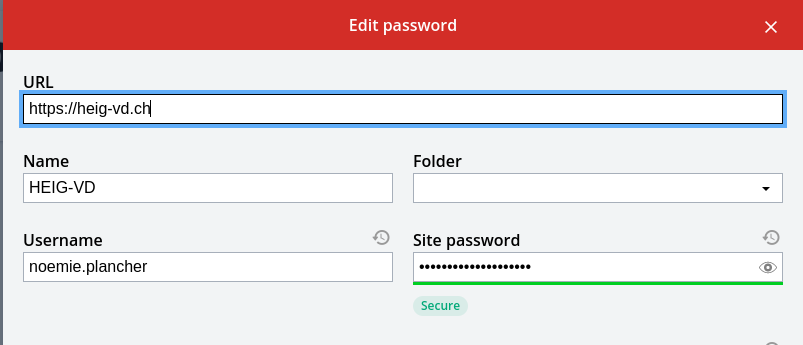
\includegraphics[width=15.5cm]{images/lp_heigvd.png}
	\caption{Identifiants pour heig-vd.ch enregistrés sur LastPass}
\end{figure}

\newpage

Ensuite, nous avons testé de nous connecter à un sous-domaine avec \\ \verb|https://webmail.heig-vd.ch|:
\begin{figure}[H]
	\centering
	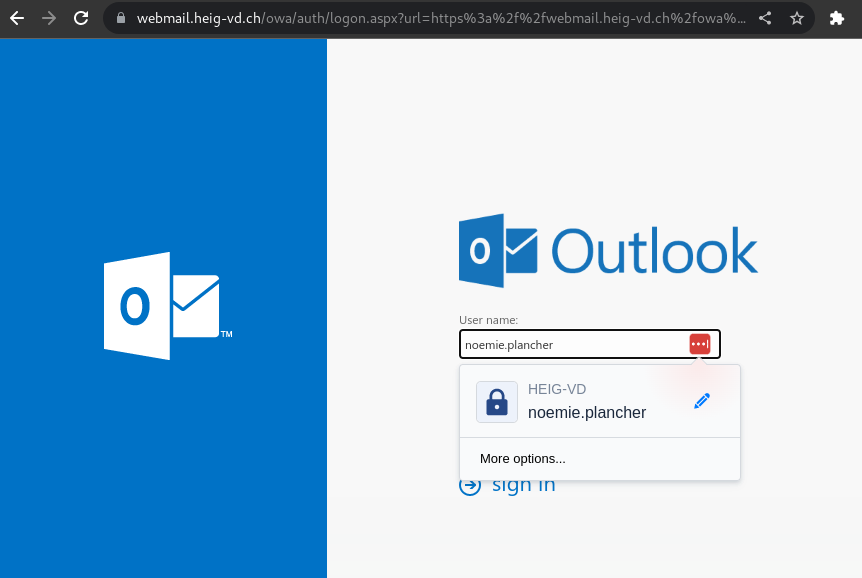
\includegraphics[width=15.5cm]{images/lp_webmail.png}
	\caption{Auto-complétion d'identifiants sur webmail.heig-vd.ch}
\end{figure}

Ainsi, nous constatons que LastPass propose les identifiants pour le sous-domaine car il les traite de la même manière.

Cette faiblesse pourrait être dangereuse car un attaquant pourrait potentiellement effectuer une attaque XSS en ajoutant un faux formulaire de connexion afin de récupérer les identifiants auto-complétés ou il pourrait utiliser l'HTML afin d'ajouter un formulaire de connexion sur le domaine client et ainsi voler des identifiants.

Néanmoins, sur LastPass, le résultat est aléatoire car la vulnérabilité n'apparaît pas pour chaque sous-domaine. En prenant notre exemple, avec le sous-domaine \verb|https://gaps.heig-vd.ch|, les identifiants ne sont pas proposés:

\begin{figure}[H]
	\centering
	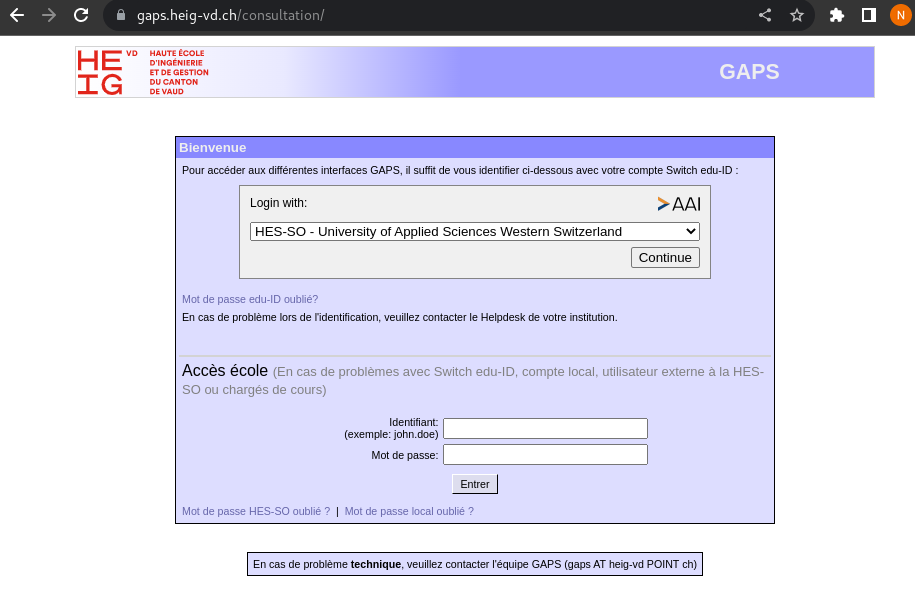
\includegraphics[width=15.5cm]{images/lp_gaps.png}
	\caption{Auto-complétion d'identifiants sur gaps.heig-vd.ch}
\end{figure}

Sinon, par défaut, LastPass auto-complète seulement les champs mais ne se connecte pas automatiquement (fonction modifiable dans les paramètres de l'entrée). Cela pourrait être critique car un attaquant pourrait effectuer une attaque XSS ou injection réseau et sans l'interaction de l'utilisateur, récupérer les identifiants qui ont été entrés dans le formulaire de connexion.

\subsection{Presse-papier}
La fonctionnalité de copier le mot de passe enregistré dans le presse-papier est souvent proposée lorsque le remplissage automatique de champs de connexion n'est pas proposée. Néanmoins, LastPass propose de copier le username, le mot de passe ou l'URL du site de connexion. 

Par défaut, LastPass nettoie le presse-papier après 60 secondes. Ce temps est correct au niveau sécurité cependant, pour une meilleure protection contre le sniffing de presse-papier, ce temps pourrait être réduit à 30 secondes maximum. L'utilisateur a également la possibilité de décocher cette case et que LastPass ne nettoie plus le presse-papier. Il est certain qu'il serait plus sécurisé d'enlever cette option afin d'éviter au maximum la perte ou le vol de données sensibles. 

Toutefois, il est compliqué de se protéger à 100\% de malwares de ce genre car à moins de ne pas permettre à l'utilisateur de copier ses mots de passe et d'effacer le presse-papier après un court instant, aucune protection n'est possible. Pour ce point, on ne peut que prévenir un maximum les utilisateurs qu'en leur exposant les risques et en leur demandant, par exemple, de verrouiller leur machine dès le moment où ils ne l'utilisent plus pour éviter qu'un attaquant sniffe leur presse-papier.
\section{Stockage}
LastPass fonctionne en ligne et hors-ligne\cite{9657969}, ainsi, il stocke des informations en local sur le disque de l'utilisateur afin d'avoir accès au coffre-fort et à toutes les données lorsque l'utilisateur n'est pas connecté à Internet. Tout dépend de l'OS et du navigateur, mais sur Windows 11 et Chrome, nous pouvons trouver une base de données SQLite à cet endroit: \\ \path{%AppData%\Local\Google\Chrome\UserData\Default\databases\chrome-extension_} 
	\\
	\path{hdokiejnpimakedhajhdlcegplioahd_0}. Nous pouvons trouver plusieurs tables différentes, dont \textit{LastPassData} où se trouvent les différentes entrées chiffrées du coffre-fort et le hash pour vérifier l'authenticité de la clé. 
	
	En se basant sur une démonstration d'attaque qui date de 2019\cite{p59}, il explique comment la fonction \textit{Remember Password} amène une vulnérabilité importante dans l'extension LastPass. Si la fonction de se rappeler le mot de passe et le mode hors-ligne sont activés, l'attaque peut réussir à récupérer le master password et le déchiffrer. Comme cité précédemment, une base de données est stockée en local chez l'utilisateur, ainsi c'est la table \textit{LastPassSavedLogins2} qui nous intéresse. Elle contient les champs suivants: username, password, last\_login, protected. En analysant le code Javascript \verb|server.js|, qui se trouve dans le fichier \verb|background.html| de l'extension, il est possible de voir comment est déchiffré le master password et ainsi écrire un script pour récupérer ce dernier en clair.
	
	Toutefois, cette attaque n'a pas pu être effectuée sur la version actuelle de l'extension car plus aucune information n'est stockée dans la table \textit{LastPassSavedLogins2}, malgré toutes les conditions remplies.
	
	\begin{figure}[H]
		\centering
		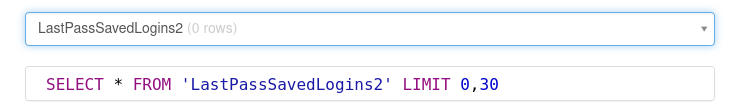
\includegraphics[width=15.5cm]{images/sql_lp.png}
		\caption{Table \textit{LastPassSavedLogins2} vide}
	\end{figure} 
	
	Nous avons analysé en profondeur le code disponible de l'extension et nous n'avons pas trouver de quelconque faiblesse qui nous permettrait de récupérer le master password enregistré. Les données qui transitent en local ont l'air d'être protégées en binaire, sans doute afin d'ajouter une couche de sécurité supplémentaire.
	
	Dès le moment où le master password n'est pas facilement récupérable et mis directement disponible pour les attaquants, cela permet de ralentir les personnes malveillantes et il est ainsi moins problématique d'avoir des données chiffrées en local.
\section{Mémoire}
D'après le whitepaper de LastPass, ils utilisent les \textit{Windows Crypto APIs}, misent à disposition par Windows, afin d'ajouter une couche supplémentaire de sécurité sur les appareils Windows. Ainsi, un test a été fait pour vérifier que le master password ou des informations sensibles, comme des mots de passe avec lesquels l'utilisateur aurait interagit, ne soient pas laissé en mémoire RAM lorsque le gestionnaire de mot de passe est verrouillé. 

Ainsi, nous avons effectué un dump de la mémoire du processus sur le disque et dû au fait que la mémoire est partiellement gérée par Windows avec ses APIs cryptographiques, il y a beaucoup de données qui sont chiffrées et illisibles. Néanmoins, avec un peu de recherche à l'aide de mes usernames que je connais, nous avons pu trouver tous les mots de passe du coffre-fort en clair dans la mémoire du processus. Nous pouvons le constater ci-dessous avec une entrée pour tumblr en recherchant le string "passworddec" sur le dump:
 
\begin{figure}[H]
	\centering
	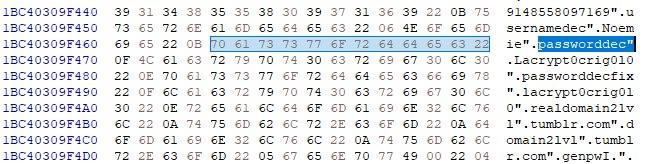
\includegraphics[width=15.5cm]{images/lp_pass.jpg}
	\caption{Entrée du coffre-fort LastPass en clair}
\end{figure} 

Cela veut donc signifier que LastPass charge tout le coffre-fort en mémoire dès que l'utilisateur se connecte et dès qu'elle est verrouillée, aucun nettoyage de la mémoire du processus n'est effectué. Toutefois, dès que le processus de l'application est stoppé, aucune donnée n'est visible en RAM.

\par\noindent\rule{\textwidth}{0.4pt}

Nous avons également effectué un autre test qui se base sur plusieurs attaques effectuées sur LastPass d'une étude de 2013\cite{zhao} et sur le travail de Bachelor de Léo Corthès\cite{leo}\footnote{Le travail étant confidentiel, il n'est pas possible de le visualiser, toutefois l'attaque expliquée s'appuie sur une étude de 2019\cite{p59}}. L'étude explique que l'extension utilise du javascript pour toutes les fonctionnalités, en incluant les opérations cryptographiques. Ainsi, la master key, qui est dérivée du master password et qui permet de chiffrer tout le coffre-fort, peut facilement se trouver dans le javscript sous le nom de variable  \verb|g_local_key|. Étant donné qu'on analyse une extension de navigateur, il est très commun d'avoir un fichier \verb|background.html| qui permet d'invoquer tous les scripts qui tournent en arrière-plan. De ce fait, en utilisant les outils de développeur sur Chrome, nous avons pu debuguer l'extension et chercher la master key pour afficher sa valeur. 

Nous avons décidé d'effectuer ce test\footnote{Les informations qui vont suivre ne seront pas censurées car il s'agit de valeurs d'exemples et non des valeurs réelles} lorsque le gestionnaire était verrouillé afin de simuler correctement une attaque possible. 

Premièrement, comme décrit dans le paragraphe plus haut, nous avons récupéré la valeur de \verb|g_local_key|, qui représente la master key, à l'aide des outils de développeur de Chrome.

\begin{figure}[H]
	\centering
	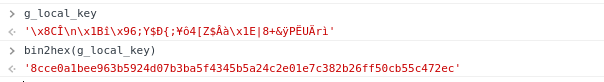
\includegraphics[width=10cm]{images/lp_master_key.png}
	\caption{Master key en mémoire}
\end{figure} 

Étant donné, que nous connaissons la valeur du master password (car il s'agit de mon compte) et que nous savons exactement comment LastPass dérive le master password (voir \ref{lp}), nous pouvons tester si la clé est réellement la master key :

\begin{lstlisting}[language=python, caption=Calcul de la master key sur LastPass]
>>> masterkey = hashlib.pbkdf2_hmac('sha256', b'Followthewhiterabbit98', b'noemie.plancherel@gmail.com', 100100, 32)
>>> binascii.hexlify(masterkey)

b'8cce0a1bee963b5924d07b3ba5f4345b5a24c2e01e7c382b26ff50cb55c472ec'

\end{lstlisting}

Ainsi, nous constatons que les deux clés sont similaires, c'est-à-dire que la variable \verb|g_local_key| est réellement la master key.

Avec cette information, nous pouvons à présent déchiffrer tout le coffre-fort. Comme précisé dans la section précédente, une base de données stocke tout le coffre-fort sur le disque de l'utilisateur. Pour cette partie, nous nous intéresserons à la table \textit{LastPassData} et au champ \textit{accts}. 

\begin{figure}[H]
	\centering
	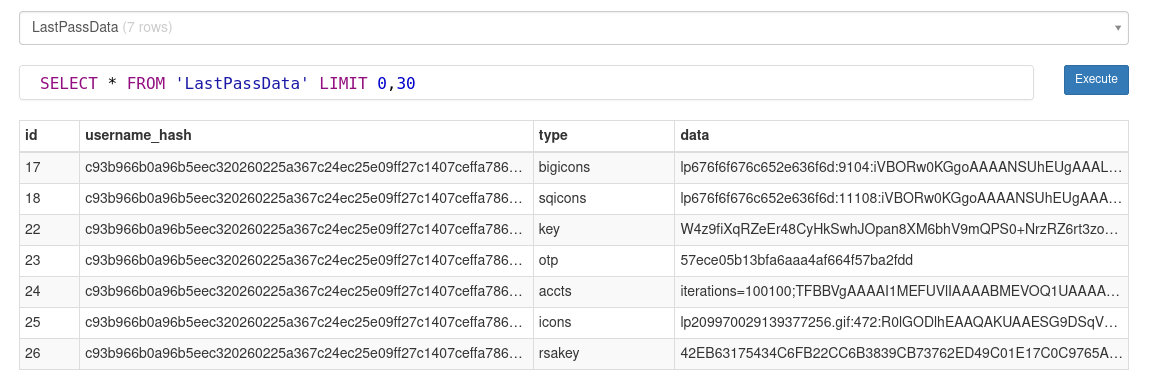
\includegraphics[width=15.5cm]{images/lp_data.png}
	\caption{Master key en mémoire}
\end{figure} 

Nous pouvons remarquer que le champ commence par le nombre d'itérations nécessaires pour dériver la master key et des données encodées en Base64 suivent. 

Les données en base64 représentent toutes les entrées du coffre-fort. L'étude de Derk Barten décrit la structure de chaque entrée qui possède des caractères de délimitations pour indiquer l'URL du site en clair, le username chiffré et le mot de passe chiffré.

Un script \ref{script_dec_lp} a été développé, inspiré par le celui proposé par Léo Corthès, afin de déchiffrer toutes les entrées du coffre-fort à l'aide de la master key récupérée à l'étape précédente. 

Toutefois, ce script a quelques limitations, il fonctionne uniquement pour les entrées basiques. LastPass propose plusieurs champs lors de l'enregistrement d'un mot de passe (username, mot de passe, URL, titre, notes ou encore un dossier). Ainsi, il est compliqué de savoir quelles entrées ont quels champs configurés et étant donné que toute la structure stockée est impactée, il n'est pas possible de déchiffrer exactement tous les champs de chaque entrée, néanmoins un maximum d'informations peuvent être récupérées sur le script, ce qui permet déjà à un attaquant d'avoir accès à quelques identifiants. 

Ces deux attaques de mémoire ont besoin de certaines conditions afin de pouvoir les exécuter sur les victimes.

\textbf{Attaque \#1 sur la mémoire du processus} 

\begin{itemize}
	\item Le gestionnaire de mot de passe doit être dans un état \textit{Locked} ou \textit{Unlocked}
\end{itemize}

\textbf{Attaque \#2 sur la mémoire du processus} 
\begin{itemize}
	\item Le gestionnaire de mot de passe doit être dans un état \textit{Unlocked}
	\item Le gestionnaire doit avoir le mode offline activé (par défaut il est activé)
	\item Le 2FA ou MFA ne doivent pas être configurés
\end{itemize}



\section{Récapitulatif de l'analyse}

Dans cette dernière section, nous allons établir un récapitulatif de toute l'analyse en passant par tous les points abordés, en ajoutant une évaluation de sécurité et en conseillant des contre-mesures nécessaires dans le cas où la faille est importante. 

% Please add the following required packages to your document preamble:
% \usepackage[table,xcdraw]{xcolor}
% If you use beamer only pass "xcolor=table" option, i.e. \documentclass[xcolor=table]{beamer}
\begin{landscape}
	\fontsize{8}{11}\selectfont
	\begin{longtable}[H]{llll}
		\cline{2-4}
		&
		\multicolumn{1}{c}{Critère analysé} &
		\multicolumn{1}{c}{Commentaire} &
		\multicolumn{1}{c}{Contre-mesures nécessaires ?} \\ \cline{2-4} 
		\cellcolor[HTML]{FFE135} &
		Master password &
		\begin{tabular}[c]{@{}l@{}}Les critères du master password sont forts,\\ cela permet de ralentir considérablement les\\ attaques de brute-force sur le master password, \\ cependant, l'entropie indique un mot de passe\\ moyen, ainsi il faudrait y faire attention pour les\\ mois à venir. Lorsque le gestionnaire est en mode \\ hors-ligne, il n'y a aucun nombre maximum \\ d'essais d'authentification, cela pourrait aider un \\ attaquant à effectuer du brute-force, néanmoins\\ étant donné que la politique des master password\\ de LastPass créée des mots de passe forts, l'attaque\\ prendrait du temps\end{tabular} &
		\begin{tabular}[c]{@{}l@{}}Il serait également bien d'ajouter un nombre d'essais \\ maximum de connexion, aussi lorsque le gestionnaire \\de mots de passe est hors-ligne, afin d'éviter au \\ maximum toute attaque de brute-force\end{tabular} \\ \hline
		\cellcolor[HTML]{228B22} &
		Chiffrement &
		\begin{tabular}[c]{@{}l@{}}L'algorithme utilisé pour le chiffrement du coffre-\\ fort est fort\end{tabular} &
		- \\ \hline 
		\cellcolor[HTML]{228B22} &
		Dérivation des clés &
		\begin{tabular}[c]{@{}l@{}}PBKDF2-SHA2 est efficace pour la dérivation \\ des clés. 100'100 rounds est également un nombre\\ assez grand pour permettre de ralentir au mieux \\ les attaques. Il serait bien d'ajouter un support pour\\ Argon2 afin de pouvoir proposer les deux\end{tabular} &
		- \\ \hline
		\cellcolor[HTML]{228B22} &
		Authentification &
		\begin{tabular}[c]{@{}l@{}}L'authentification auprès des serveurs est implémentée\\ de sorte à ce qu'il soit difficile de se faire passer par\\ l'utilisateur sans connaître son master password\end{tabular} &
		- \\ \hline
		\cellcolor[HTML]{228B22} &
		\begin{tabular}[c]{@{}l@{}}Génération de \\ mots de passe\end{tabular} &
		\begin{tabular}[c]{@{}l@{}}Les résultats sont plutôt bons; des mots de passes \\ faibles sont très occasionnellement générés et ils ont\\ de bons score au niveau du nombre d'essais pour les \\ deviner.\end{tabular} &
		\begin{tabular}[c]{@{}l@{}}Étant donné que par défaut, LastPass génère  des mots de passe \\ de 12 caractères, il serait bien de l'augmenter d'au moins 14 \\ caractères. De plus, il serait bien d'ajouter des symboles en plus de \\ ceux proposés afin de garantir un très bon aléatoire\end{tabular} \\ \hline
		\cellcolor[HTML]{FF9933} &
		Auto-complétion &
		\begin{tabular}[c]{@{}l@{}}Nous avons pu constater que des failles de 2013 sont\\ toujours présentes sur LastPass, notammant en ignorant\\ les sous-domaines lors de l'auto-complétion des champs.\\ L'option auto-remplissage des champs peut également\\ être dangereuse et être vulnérable à des attaques où un \\ attaquant ajouterait un formulaire de connexion caché.\end{tabular} &
		\begin{tabular}[c]{@{}l@{}}Une meilleure comparaison d'origine lors de l'auto-remplissage des \\ champs de formulaire serait nécessaire pour éviter toutes attaques. \\ De plus, l'option de auto-remplissage des champs étant activée \\ par défaut lors d'ajout d'une entrée dans le coffre-fort, il serait \\mieux de la désactiver et de laisser le choix à l'utilisateur ou d'avoir \\ une interaction avec ce dernier avant de remplir le champ pour \\qu'il puisse valider\end{tabular} \\ \hline
		\cellcolor[HTML]{228B22} &
		Presse-papier &
		\begin{tabular}[c]{@{}l@{}}Le timeout ajouté lors de la copie d'identifiants est correct.\\ Peut-être que baisser ce temps à 30-40 secondes serait\\ une meilleure solution, cependant il est compliqué de \\ se protéger à 100\% des attaques de sniffing, mais LastPass\\ ne peut rien faire de plus.\end{tabular} &
		- \\ \hline 
		\cellcolor[HTML]{FFE135} &
		Stockage &
		\begin{tabular}[c]{@{}l@{}}La base de données stockée local ne contient aucune \\ information en clair qui serait facile de récupérer directement.\\ La fonction de se rappeller du master password est sécurisée\\ car il n'y a pas la possibilité de récupérer le master password\\ directement dans une table de la base de données.\end{tabular} &
		\begin{tabular}[c]{@{}l@{}}En liaison avec les failles découvertes dans la  mémoire, il serait\\ nécessaire de désactiver le mode offline par défaut afin d'éviter \\ d'avoir des fichiers en local chez l'utilisateur. Cependant, sur \\LastPass afin de pouvoir désactiver ce mode, il faut avoir le 2FA \\ou MFA activé sur le gestionnaires. Ainsi, il faudrait également \\dissocier ces deux options.\end{tabular} \\ \hline
		\cellcolor[HTML]{CE2029} &
		Mémoire &
		\begin{tabular}[c]{@{}l@{}}Nous avons découvert deux failles assez critiques liées à la\\ mémoire et également au stockage de la base de données en \\ local. Premièrement, même quand le gestionnaire de mot de \\ passe est verrouillé, on a la possibilité de récupérer tous les\\ identifiants, avec mots de passe, en clair dans la mémoire du\\ processus car LastPass semble charger tout le coffre-fort en \\ mémoire et l'efface quand le processus est terminé. La seconde\\ faille permet de récupérer la master key depuis les outils de\\ développeurs de Chrome et de déchiffrer une grande partie du\\ coffre-fort grâce aux données stockées en local.\end{tabular} &
		\begin{tabular}[c]{@{}l@{}}La première faille est très critique, étant donné qu'un\\ attaquant pourrait effectuer un dump de la mémoire\\ assez facilement, même quand le gestionnaire de mots de\\ passe est verrouillé et il n'a pas besoin de privilèges\\ pour effectuer l'attaque. La sécurité à ajouter serait dans\\ un premier temps de s'assurer de nettoyer la mémoire\\ dès que le gestionnaire est verrouillé, puis s'assurer que\\ les données sensibles, tels que les mots de passe, soient\\ chiffrés dans la mémoire du processus, pour cela les OS\\ mettent à dispositon des APIs de cryptographie. De plus,\\ un timeout de session pour verrouiller le gestionnaire \\ après un certain temps serait une très bonne couche\\ sécuritaire en plus. Pour la seconde attaque, la première\\ contre-mesure à prendre serait de désactiver par défaut\\ le mode offline. Puis au niveau des outils de développeurs\\ de Chrome, il est assez difficile de gérer cette partie car\\ cela touche à tout l'arrière-plan de l'extension qui est \\ nécessaire quant à l'utilisation du gestionnaire.\end{tabular} \\ \hline
		\cellcolor[HTML]{FFE135} &
		Divers &
		\multicolumn{2}{l}{\begin{tabular}[c]{@{}l@{}}Nous pouvons ajouter un commentaire sur un élément que nous n'avons pas analysé mais qui est très important\\ à commenter; par défaut, l'extension ne se verrouille jamais, même quand le processus se termine. C'est à l'utilisateur \\ de se déconnecter manuellement. Cela pourrait être critique de ne jamais stopper la session, car un attaquant qui a accès \\au device déverrouillé de l'utilisateur, aura également accès au coffre-fort et à toutes les données en clair. Afin d'éviter \\ au maximum un vol de données, il serait recommandé d'ajouter un timeout de session par défaut (car actuellement il \\ est possible de le configurer dans les paramètres de LastPass).\end{tabular}} \\ \hline
		&
		&
		&
		\\
		\multicolumn{4}{l}{\textcolor{forestgreen(web)}{$\blacksquare$} Bonne sécurité, aucun contre-mesure à ajouter \textcolor{bananayellow}{$\blacksquare$} Sécurité moyenne, points à faire attention et quelques recommandations au niveau des contre-mesures} \\
		\multicolumn{4}{l}{\textcolor{deepsaffron}{$\blacksquare$} Sécurité faible, contre-mesures à prendre \textcolor{fireenginered}{$\blacksquare$} Sécurité très faible, contre-mesures à prendre rapidement car failles critiques} \\		      
	\end{longtable}
\end{landscape}

% +---------------------------------------------------------------+
% | Author :    Sylvain Pasini, HEIG-VD
% | Date :       June 3rd, 2021
% +---------------------------------------------------------------+


\chapter{Conclusion}



% +---------------------------------------------------------------+
%\backmatter

\cleardoublepage
\phantomsection
\addcontentsline{toc}{chapter}{Bibliographie}
\bibliographystyle{plain}
\bibliography{chapters/biblio}
\nocite{*} %ajoute tout ce qu'il y a dans le bibtex

\cleardoublepage
\phantomsection
\addcontentsline{toc}{chapter}{Liste des figures}
\listoffigures

\cleardoublepage
\phantomsection
\addcontentsline{toc}{chapter}{Liste des tableaux}
\listoftables

\cleardoublepage
\phantomsection
\addcontentsline{toc}{chapter}{Liste des listings}
%\listoflistings
\tcblistof[{\chapter*}]{mypyg}{Liste des listings}


% Annexes
% +---------------------------------------------------------------+
\appendix

% +---------------------------------------------------------------+
% | Author :    Sylvain Pasini, HEIG-VD
% | Date :       June 3rd, 2021
% +---------------------------------------------------------------+


\chapter{Journal de travail}

\begin{landscape}

\begin{longtable}[c]{lp{10cm}rrrr}
    \caption{Journal de travail}\\

    \hline
    Date & Description & Rech. [h] & Dev. [h] & Rapport [h] & Admin [h] \\
    \hline
    \endfirsthead
    
    \hline
    Date & Description & Rech. [h] & Dev. [h] & Rapport [h] & Admin [h] \\
    \hline
    \endhead
    
    \multicolumn{6}{r}{\small \it Le journal de travail continue à la page suivante.} \\
    \normalsize
    \endfoot
    
    \hline
    \endlastfoot


  % Work
    > 20.09.22
    & Discussion avec le professeur responsable, établissement du cahier des charges, introduction
    & 7 %recherche
    & 0 %dev
    & 10 %reporting
    & 4\\ %admin
    
	20.09.2022 
	& Update + organisation du TB, planing, relire le début du TB déjà commencé, avancement de l’étude du marché (fonctionnalités, plateformes, prix), lecture d’articles
	& 2 %recherche
	& 0 %dev
	& 5 %reporting
	& 1\\ %admin

	21.09.2022 
	& Recherches sur les statistiques des gestionnaires de mots de passe sur le marché, rédaction du chapitre étude de marché (terminé ce jour-ci)
	& 3 %recherche
	& 0 %dev
	& 3 %reporting
	& 0\\ %admin

	22.09.2022
	& Introduction et organisation du chapitre étude sécuritaire, recherche et lecture sur les différentes implémentations sécuritaire des gestionnaires de mots de passe
	& 3 %recherche
	& 0 %dev
	& 1 %reporting
	& 1\\ %admin

	23.09.2022 
	& Recherche et lecture sur les différentes implémentations sécuritaire des gestionnaires de mots de passe et organisation du rapport
	& 1 %recherche
	& 0 %dev
	& 1 %reporting
	& 0\\ %admin

	26.09.2022  
	& Recherche et lecture sur les gestionnaires de mots de passe browser-based, rédaction dans le rapport à ce propos
	& 4 %recherche
	& 0 %dev
	& 1 %reporting
	& 0\\ %admin
	
	
	27.09.2022  
	& Recherche et lecture sur les gestionnaires de mots de passe browser-based et local-based, et rédaction dans le rapport
	& 3 %recherche
	& 0 %dev
	& 2 %reporting
	& 0\\ %admin
	
	28.09.2022  
	& Recherche et lecture sur les gestionnaires de mots de passe browser-based et local-based, et rédaction dans le rapport
	& 4 %recherche
	& 0 %dev
	& 1 %reporting
	& 0\\ %admin

	29.09.2022  
	& Recherche et lecture sur les gestionnaires de mots de passe local-based, et rédaction dans le rapport
	& 5 %recherche
	& 0 %dev
	& 3 %reporting
	& 0\\ %admin

	30.09.2022 
	& Rédaction de la section du partage d'informations, des 3 états du gestionnaires de mots de passe 
	& 1 %recherche
	& 0 %dev
	& 4 %reporting
	& 0\\ %admin

	03.10.2022 
	& Fin du chapitre 3 sur analyse de menaces, lecture sur la modélisation de menaces et la norme que je souhaite suivre
	& 7 %recherche
	& 0 %dev
	& 1 %reporting
	& 0\\ %admin

	04.10.2022
	& Début chapitre analyse de menaces et lecture de la norme choisie
	& 6 %recherche
	& 0 %dev
	& 2 %reporting
	& 0\\ %admin
	
	05.10.2022
	& Lecture et rédaction établissement du contexte de l'analyse de menaces
	& 5 %recherche
	& 0 %dev
	& 3 %reporting
	& 0\\ %admin

	06.10.2022 
	& Lecture et rédaction établissement du contexte de l'analyse de menaces
	& 2 %recherche
	& 0 %dev
	& 6 %reporting
	& 0\\ %admin

	07.10.2022 
	& Lecture et rédaction identification des risques de l'analyse de menaces
	& 5 %recherche
	& 0 %dev
	& 3 %reporting
	& 0\\ %admin

	09.10.20220 
	& Lecture et rédaction identification des risques de l'analyse de menaces
	& 2 %recherche
	& 0 %dev
	& 2 %reporting
	& 0\\ %admin
	
	10.10.20220 
	& Lecture et rédaction identification des risques de l'analyse de menaces
	& 3 %recherche
	& 0 %dev
	& 5 %reporting
	& 0\\ %admin
	
	11.10.20220 
	& Rédaction et lecture analyses des risques et évaluation des risques
	& 4 %recherche
	& 0 %dev
	& 4 %reporting
	& 0\\ %admin
	
	12.10.20220 
	& Rédaction et lecture analyses des risques et évaluation des risques
	& 3 %recherche
	& 0 %dev
	& 4 %reporting
	& 0\\ %admin
	
	13.10.20220 
	& Rédaction du traitement des risques et lecture à ce propos avec les contremesures possibles
	& 3 %recherche
	& 0 %dev
	& 3 %reporting
	& 0\\ %admin
	
	14.10.20220 
	& Rédaction de la section exigences sécuritaires à respecter, relecture du TB, organisation du rapport et rendu intermédiaire du rapport
	& 1 %recherche
	& 0 %dev
	& 6 %reporting
	& 0\\ %admin

	16.10.20220
	& Rédaction de la sélection des candidats
	& 2 %recherche
	& 0 %dev
	& 6 %reporting
	& 0\\ %admin
	
\end{longtable}


\end{landscape}


\end{document}

% Auteur : Sylvain Pasini, HEIG-VD, 2021
